%%%%%%%%%%%%%%%%%%%%%%%%%%%%%%%%%%%%%%%%%%%%%%%%%%%%%%%%%%%%%%%%%%%%%%%%%%%%%%%%%%%%%%%%%%%%%%%%%%%%%%%%%%%%%%%%%%%%%%%%%%%%%%%%%%%%%%%%%%%%%%%%%%%%%%%%%%%
% This is just an example/guide for you to refer to when submitting manuscripts to Frontiers, it is not mandatory to use frontiers.cls nor frontiers.tex  %
% This will only generate the Manuscript, the final article will be typeset by Frontier after acceptance.                                                 %
%%%%%%%%%%%%%%%%%%%%%%%%%%%%%%%%%%%%%%%%%%%%%%%%%%%%%%%%%%%%%%%%%%%%%%%%%%%%%%%%%%%%%%%%%%%%%%%%%%%%%%%%%%%%%%%%%%%%%%%%%%%%%%%%%%%%%%%%%%%%%%%%%%%%%%%%%%%

%%% Version 2.0 Generated 2013/09/12 %%%
%%% You will need to have the following packages installed: datetime, fmtcount, etoolbox, fcprefix, which are normally inlcuded in WinEdt. %%%
%%% In http://www.ctan.org/ you can find the packages and how to install them, if necessary. %%%

\makeatletter
\adddialect\l@English\l@english
\makeatother

%\documentclass{frontiersENG} % for Engineering articles
\documentclass[english]{frontiersSCNS} % for Science articles
%\documentclass{frontiersMED} % for Medicine articles

\usepackage{url,lineno}
\linenumbers

\newtheorem{definition}{Definition}

\usepackage{graphicx}
\usepackage[english]{babel}
%It ensures a direct compilation from tex to pdf.
\usepackage{epstopdf}
%\usepackage[sort, numbers, authoryear]{natbib}
\usepackage{listings}
\usepackage{amsmath}
\usepackage{longtable}
\usepackage{url}
\usepackage{flushend}
\usepackage{algorithm}
%\usepackage{algorithmic}
\usepackage{algpseudocode}
%\usepackage{algorithmicx}
\usepackage{caption}% http://ctan.org/pkg/caption
\usepackage{lscape}
\usepackage{subfig}
\usepackage{etoolbox}
\apptocmd{\sloppy}{\hbadness 10000\relax}{}{}


% Leave a blank line between paragraphs in stead of using \\

\copyrightyear{}
\pubyear{}

\def\journal{Neuroinformatics}%%% write here for which journal %%%
\def\DOI{}
\def\articleType{Research Article}
\def\keyFont{\fontsize{8}{11}\helveticabold }
\def\firstAuthorLast{Je\v{z}ek {et~al.}} %use et al only if is more than 1 author
\def\Authors{Petr Je\v{z}ek\,$^{1,*}$, Roman Mou\v{c}ek\,$^{2}$}
% Affiliations should be keyed to the author's name with superscript numbers and be listed as follows: Laboratory, Institute, Department, Organization, City, State abbreviation (USA, Canada, Australia), and Country (without detailed address information such as city zip codes or street names).
% If one of the authors has a change of address, list the new address below the correspondence details using a superscript symbol and use the same symbol to indicate the author in the author list.
\def\Address{$^{1,2}$New Technologies for the Information Society, Department of Computer Science and Engineering, University of West Bohemia, Plze\v{n} Czech Republic}
% The Corresponding Author should be marked with an asterisk
% Provide the exact contact address (this time including street name and city zip code) and email of the corresponding author
\def\corrAuthor{Petr Je\v{z}ek}
\def\corrAddress{New Technologies for the Information Society, Department of Computer Science and Engineering, Faculty of Applied Sciences, University of  West Bohemia, Univerzitn\'{i} 8, 306 14  Plze\v{n}, Czech Republic}
\def\corrEmail{jezekp@ntis.zcu.cz}

% \color{FrontiersColor} Is the color used in the Journal name, in the title, and the names of the sections.

\sloppy
\begin{document}
\onecolumn
\firstpage{1}

\title[Mapping Object-Oriented Structures to Semantic Web Technologies]{Semantic Framework for Mapping Object-Oriented Structures to Semantic Web Technologies}
\author[\firstAuthorLast]{\Authors}
\address{}
\correspondance{}
\extraAuth{}% If there are more than 1 corresponding author, comment this line and uncomment the next one.
%\extraAuth{corresponding Author2 \\ Laboratory X2, Institute X2, Department X2, Organization X2, Street X2, City X2 , State XX2 (only USA, Canada and Australia), Zip Code2, X2 Country X2, email2@uni2.edu}
\topic{}% If your article is part of a Research Topic, please indicate here which.

\maketitle

%%%%%%%%%%%%%%%%%%%%%%%%%%%%%%%%%%%%%%%%%%%%%%%%%%%%%%%%%%%%%%%%%%%%%%%%%%%%%%%%%%%%%%%%%%%%%%%%%%%%%%%%%%%%%%%%%%%%%%%%%%%%%%%%%%%%%%%%%%%%%%%%%%%%%%%%%%%%%%%%%%%%%%%%%%%%%%%%%%%%%%%%%%%%%%%%%%%%%%%%%%%%%%%%%%%%%%%%%%%%%%%%%%%%%%%
%%% The sections below are for reference only.
%%%
%%% For Original Research Articles, Clinical Trial Articles, and Technology Reports the following sections are mandatory:
%%% Abstract, Introduction, Material and Methods, Results, and Discussion.
%%% Please note that the Material and Methods section can be placed in any of the following ways: before Results, before Discussion or after Discussion.
%%%
%%% For Clinical Case Studies the following sections are mandatory: Abstract, Introduction, Background, Discussion, and Concluding Remarks.
%%%
%%% For all other article types there are no mandatory sections.
%%%%%%%%%%%%%%%%%%%%%%%%%%%%%%%%%%%%%%%%%%%%%%%%%%%%%%%%%%%%%%%%%%%%%%%%%%%%%%%%%%%%%%%%%%%%%%%%%%%%%%%%%%%%%%%%%%%%%%%%%%%%%%%%%%%%%%%%%%%%%%%%%%%%%%%%%%%%%%%%%%%%%%%%%%%%%%%%%%%%%%%%%%%%%%%%%%%%%%%%%%%%%%%%%%%%%%%%%%%%%%%%%%%%%%%

\begin{abstract}

%%% Leave the Abstract empty if your article falls under any of the following categories: Editorial Book Review, Commentary, Field Grand Challenge, Opinion or specialty Grand Challenge.
\section{}
   A lot of laboratories around the world deal with electrophysiology research and produce vast amounts of experimental data and related metadata. A variety of experimental approaches, used techniques, targeted subjects, usable hardware and software infrastructures etc. lead to the accumulation of data that are stored in various, often proprietary, data formats,  and annotated differently in both scope and quality sense. Moreover, the data are stored in various repositories including files and databases of different types and annotated respecting limitations of used technologies. Taken into account these conceptual and technological heterogeneities and not giving up efforts to increase research efficiency in the field by sharing data resources among laboratories the long term management and sharing of experimental data and metadata are crucial tasks. Improvement of data sharing requires to provide data in standardized data formats and related metadata in standardized semantic structures. The abstract level of such data formats and semantic structures that on one hand should bring real sharing opportunities to the domain and on the other hand which would not hinder anyone from the community to produce data in these formats and structures are currently widely discussed in the community. The next step is to provide expressive means that promote the data sharing and the third steps is to cope with the current reality. Although storing data in semantic repositories have become more popular in the last years, most of the data is stored in conventional repositories such as files and relational databases. If shared these data repositories are, for obvious reasons, designed as read-only for third party subjects and only data owners are entitled to add any semantics to the presented metadata. Moreover, conventional data repositories due to their limitations in semantic expressivity exclude to add more complex semantic information. To cope with both these opportunities we introduced a solution that enables to add additional semantics directly in the code that processes conventional data repositories. This approach should not burdensome users with additional demands on programming environment. That is why this was done by using reflective Java annotations, syntactic metadata that are added to Java source code and retrieved at run-time. Moreover, this semantics need not to be written directly by the programmer directly to the code, but it can be collected from non-programmers using a graphic user interface.
   
   This sand it is not possible to add there any semantic information that could be found later. The goal of this paper is to introduce the wato include additional semantics into data descriptions that To improve the data sharing  The Various experimental leads to  experiments a crucial task in e. The complexity of data and their heterogeneous nature makes the data unsustainable. When the data description is improved, its sharing and management will be more effective. Although scientific communities have been intensively working on description of data from individual neuroscience domains by domain ontologies, which can be expressed by Semantic Web languages, current neuroinformatics tools use script-based programming languages, and what more, large, robust and fault-tolerant systems, intended for data sharing, are object-oriented. As a result, a suitable mapping between object-oriented systems and Semantics Web systems has to be ensured.  The paper presents a developed mapping that enables transformation of common object-oriented code into the Semantic Web descriptions. Furthermore, an annotation-based approach is proposed to particularly solve the problem of the described semantic gaps. The proposed mapping is practically implemented as a library - the Semantic Framework. Finally, integration of the Semantic Framework in the EEG/ERP Portal, together with its registration in the Neuroscience Information Framework, validates the presented approach.
\tiny
 \keyFont{ \section{Keywords:} EEG/ERP experiment, Object-oriented code, Semantic web, Ontology, Concepts mapping, Semantic Framework} %All article types: you may provide up to 8 keywords; at least 5 are mandatory.
\end{abstract}

\section{Introduction}
\label{intro}
Our research group specializes in brain activity research. Experiments are focused on measurement of reaction times of drivers, motor skills of children, or mouse blindness. We use methods of Electroencephalography (EEG) and its subdomain Event-Related Potentials (ERP). Measurement of EEG/ERP experiments is a time-consuming task that produces a lot of data. When the number of experiments increases, the need to find a mature system for data sharing and management also increases. Although many laboratories deal with data collecting, their long-term storage is not satisfactorily solved. The most pressing difficulty is an absence of standardized and generally used data formats. The data formats should describe not only raw data, but researchers even more emphasize the need to provide a well-defined metadata description \cite{data-sharing-for-computational-neuroscience}. These initiatives cover the International Neuroinformatics Coordinating Facility (INCF), formed in 2005 \citep{INCF-evaluation-first-year}. INCF is developing an infrastructure serving its national nodes which are responsible for partial infrastructures in specific domains.

Although, domain ontologies that have played a significant role in information systems \citep{747902} are well-designed for heterogeneous data description, software systems that deal with large data collections are almost exclusively object-oriented;  data are stored in relational databases. The semantic gaps between an object-oriented code and Semantic Web languages (that are used for expressing domain ontologies) are significant and their resolution is crucial.

The main contribution of this paper is a proposed mapping and its implementation that extends a common object-oriented code with missing semantics. The proposed mapping is practically implemented within the Semantic Framework presented in Section \ref{Semantic_Framework}.

The presented approach is discussed from performance (Section \ref{Performance_evaluation}) and usability (Section \ref{discussion}) perspectives. The performance tests measure the rate of transformation with increasing number of instances. The usability verification is based on the following use-case study:

First, an ontology (Section \ref{Experimental_Ontology}) describing EEG/ERP experiments was designed.

Second, the implementation of the ontology (Section \ref{Implementation-within-EEG-ERP-Portal}) and integration of the Semantic Framework (Section \ref{Semantic_Framework_Integration_with_EEG_ERP_Portal}) in a system intended for storing, sharing and interchange of EEG/ERP experiments, the EEG/EERP Portal, is presented.

Last, registration of the generated ontology document in the Neuroscience Information Framework (NIF) demonstrates searchability of stored data using a unified interface (Section \ref{Registration_within_nif}).


\section{Related Work}
\label{Related_Work}

Several approaches and tools that try to map a relational schema or an object-oriented code to the Semantic Web or back exist. Some of these approaches exist only as initial proposals or prototypes described in scientific papers, while some of them have been really implemented as available frameworks.

\subsection{Relational Schema and RDF}
\label{Relational_Schema_RDF}

A familiar representation of an RDF fact might be represented as a row in a table in a relational database. This table has two columns, corresponding to the subject and the object of the RDF triple. The name of the table corresponds to the predicate of the RDF triple. In this table each row represents a unique instance of the subject. Such a row has to be decomposed for representation as RDF triples \citep{0123820200, 4811327}.

The D2RQ \citep{efeliksik:bizer2004d2rq} is a framework that uses declarative language to describe mappings between relational database schema and RDF. The D2RQ Platform provides possibilities
to query a non-RDF database using the SparQL \citep{prudhommeaux2008sparql} query language, to access information in a non-RDF database using the Jena API or the Sesame API \citep{sryll:conf/iswc02/sesame}.

METAMorphoses \citep{svihla} is a data transformation processor from RDB into RDF that uses the mapping described in the template XML document. The XML template defines a set of mapping rules and queries for obtaining data stored in a relational database.

\subsection{Object-Oriented Model and OWL}
\label{OOM-and-OWL}

\subsubsection{Tool with Common Semantic Expressivity}
\label{Tools_With_Common_Semantic_Expressivity}

We tested several approaches that provided limited possibilities to map common syntaxes of an object-oriented code to an OWL representation. These tools map fundamental OWL features. This means that only the basic semantic expressivity of OWL is used. Mapping of OWL classes to Java Interfaces is described in \citep{sryll:conf/seke04/owl-mapping}. Mapping a Java Interface instead of a common Java class enables the expression of the multiple inheritance of OWL properties. Back transformation is described in \citep{Koide_owlvs.}, where the OWL processor SWCLOS3, which is at the top of the Common Lisp Object System (CLOS), is described. Whereas CLOS allows lisp programmers to develop Object-Oriented systems, SWCLOSS allows programmers to construct domain and task ontologies in software application fields.

Java2OWL-S \citep{DBLP:conf/ic3k/Ohlbach12} is a tool which is able to generate OWL directly. It uses two transformations. The first transformation is from JavaBeans into WSDL (Web Service Description Language). The input of this transformation is formed by a Java class and the output is a temporary WSDL file. The second transformation generates OWL from the WSDL file.

\subsubsection{Tool with Additional Semantic Expressivity}
\label{Tools_With_Additional_Semantic_Expressivity}


Concerning one-side transformations, the tools described in \ref{Tools_With_Common_Semantic_Expressivity} work quite satisfactorily because object-oriented code has poorer semantics than OWL. However, in these tools, no possibility to enrich the object-oriented code with missing semantics exists.

The ActiceRDF \citep{ActiveRDF} is a library for accessing RDF data from Ruby programs. It provides a domain-specific language for RDF models; it can address
RDF resources, classes and properties programmatically. When a dynamic interpreted language is used, data types are evaluated in runtime, so they can be changed dynamically.

The Semantic Object Framework (SOF) \citep{SOF} utilizes embedded comments in source codes to describe semantic relationships between classes and attributes.

The eClass \citep{Web-Information-Representation} is a solution that changes Java syntax to embed semantic descriptions into the source code.

Tested frameworks try to enrich the input object-oriented code by missing semantics using either embedded comments or changing the JavaBean syntax. The usage of such
tools is difficult because it requires a modified compiler and Java interpreter. The limitations of tested frameworks motivate us to provide a proprietary solution that will use common programming features and resolve semantic gaps in maximal range.


\section{Systems for Data Modeling}
\label{Systems for Data Modeling}

\subsection{Common Systems}
\label{Common_Systems}

Several ways to represent data in electrophysiology exist. The popularity of script-based languages is rising in neuroinformatics \citep{10.3389/neuro.11.014.2009}. Programming languages such as Matlab or Python are easy to use due to, e.g., simple data types, dynamic typing of variables or interpreted compilation. On the other hand, these languages are not suitable for development of large systems \citep{Scott:2004:PGB:1040231.1040267}.

After analyzing several semantic data models \citep{0720407583, 0126445516}, essentially the following data modeling formalisms are widely used: \emph{the entity-relationship-attribute (ERA)} model and \emph{object-oriented (OO)} model. Newer approaches, e.~g. \emph{Enhanced-entity�-relationship (EER)} model, only combine two approaches discussed above.


\subsection{Semantic Web Modeling}
\label{Semantic_Web_Modeling}

Because of the World Wide Web (WWW) contains a large collection of unclassified information, it is extremely difficult to handle this enormous amount of information. 
A promising approach, the Semantic Web \citep{bernerslee2001semantic}, represents web content in a form that is more easily machine-processable. Intelligent techniques deriving semantic relationships are developed by research groups \citep{The-Semantic-Web-ISWC-2002}. When a higher semantic expressivity is required, the semantic relationships have to be added manually.

\subsection{Concepts Discussion}
\label{Concepts_discussion}
The concepts based on semantic web languages provide appropriate features to describe data semantics. On the other hand, the Semantic Web languages are not popular for developing application programs \citep{Semantic_Web_Primer}. We believe that we can profit from a combination of both object-oriented and semantic concepts by designing a robust object-oriented system storing data in a relational database. A superstructure that provides semantic description of relationships among data can be implemented using the Semantic Web languages.


\section{Mapping Data Models}
\label{Mapping_Data_Models}

\subsection{Basic Data Concepts}
\label{Data_Concepts}
The pilar relational databases are entities and their relations; a similar representation exists in object-oriented modeling (OOM).

The Semantic Web expresses data by a triple-oriented language, \emph{Resource Description Framework (RDF)} \citep{wnpx:RDF-PRIMER}. Because expressivity of RDF is limited, W3C\footnote{http://www.w3.org/} defined a more powerful language with more capabilities for expressing meaning and semantics, \emph{Web Ontology Language (OWL)} \citep{jahrynx:Dean:04:OWO}. Three sublanguages of OWL are defined. The most restricted is OWL Lite, while OWL DL is its superset. The largest set of primitives contains OWL Full, which is a superset of both \citep{McGuinness:2004}.

\subsection{Concepts Comparison}
\label{concepts_comparison}


The OWL concepts \citep{owl2-overview} are several types according to their semantic meaning. The concepts are either properties of class restrictions or class axioms, or they can define a relation of a property to other properties, or they can be a part of an ontology header.

Semantic Web technologies associate three types of features used in the object-oriented world. They describe reality on the conceptual level independent of technological restrictions, i. e. they are similar to UML representations in OOP. They also constitute a database schema for the base of facts (RDF). Eventually they are processed by software tools in the implemented application, i. e. they are part of the implementation.

At first sight there are several similarities between UML and OWL. They both have classes, instances or inheritance. Both also enable defining cardinality restrictions, etc.

However, in a more detailed view there are many differences. The most substantial difference is the meaning of properties and individuals. In UML instances and properties are removed from classes; in OWL, properties are double types; object and datatype properties. The first one links an individual to an individual and the second one links individuals to data values. Next, UML properties always belong to a class, while OWL properties are stand-alone entities. Finally, an understanding of a class extent is also different. While UML classes work inside a program where they are defined, the OWL classes provide features to share classes among domains.

OWL classes may be defined as a set of individuals which satisfy a restriction expression. Restrictions are two types: either a boolean combination of other classes (\emph{Intersection, Union, Complement}) or a property value restriction on properties (\emph{allValuesFrom, someValuesFrom}).

OWL can discipline names using \emph{AllDifferent}, \emph{SameAs} or \emph{DifferentFrom} constructs. \emph{The Ontology Definition Metamodel} \citep{OMG2009} compares concepts of OWL with the features of UML more in depth.

Described differences are summarized in Table \ref{tab:OWL-and-UML-Features-Comparison} and practically demonstrated in Figure \ref{fig:umlowlexample}. A need for open research tools has been identified \citep{Ince2012}, therefore we selected Java as a typical example of open-source object-oriented programming language.

\begin{landscape}
% For tables use
\begin{table}
% table caption is above the table
\caption{OWL and UML Features Comparison}
\label{tab:OWL-and-UML-Features-Comparison}       % Give a unique label
% For LaTeX tables use

\begin{tabular}{p{5cm}p{4cm}p{5cm}p{5cm}}
\hline\noalign{\smallskip}
\textbf{UML} & \textbf{OWL} & \textbf{Java} & \textbf{Comment}
\\
\hline\noalign{\smallskip}
Class, atomic type, property ownedAttribute & owl:Class & \emph{class} &
\\
\hline\noalign{\smallskip}
instance & individual & class instance & OWL owl:individual class independent
\\
\hline\noalign{\smallskip}
owned attribute, association & owl:DataTypeProperty, owl:ObjectProperty & class attributes: primitive data types/objects & OWL has only global attributes
\\
\hline\noalign{\smallskip}

subclass, generalization & owl:subclass, owl:subproperty & \emph{extends}, inherited classes and properties & Java does not support multiple inheritance
\\
\hline\noalign{\smallskip}

enumeration & owl:oneOf & \emph{enum} &
\\
\hline\noalign{\smallskip}

disjoint & owl:disjointWith, owl:unionOf & One object always an instance of exactly one class, but we should pay attention to class inheritance &
\\
\hline\noalign{\smallskip}

multiplicity & owl:MinCardinality, owl:MaxCardinality & \multicolumn{1}{c}{---} &
\\
\hline\noalign{\smallskip}

package & ontology & \emph{package} &
\\
\hline\noalign{\smallskip}
dependency & RDF:property & methods parameters or return value &
\\
\hline\noalign{\smallskip}
\multicolumn{1}{c}{---} & owl:intersectionOf, owl:unionOf, owl:complementOf, owl:DifferentFrom, owl:AllDifferentFrom, owl:allValuesFrom, owl:someValuesFrom, owl:SameAs & \multicolumn{1}{c}{---} &
\\
\hline\noalign{\smallskip}
\end{tabular}

\end{table}

\end{landscape}

\begin{figure}
% Use the relevant command to insert your figure file.
% For example, with the graphicx package use
\begin{tabular}{c}
  \subfloat[Definitions of classes with primitive and object properties.]{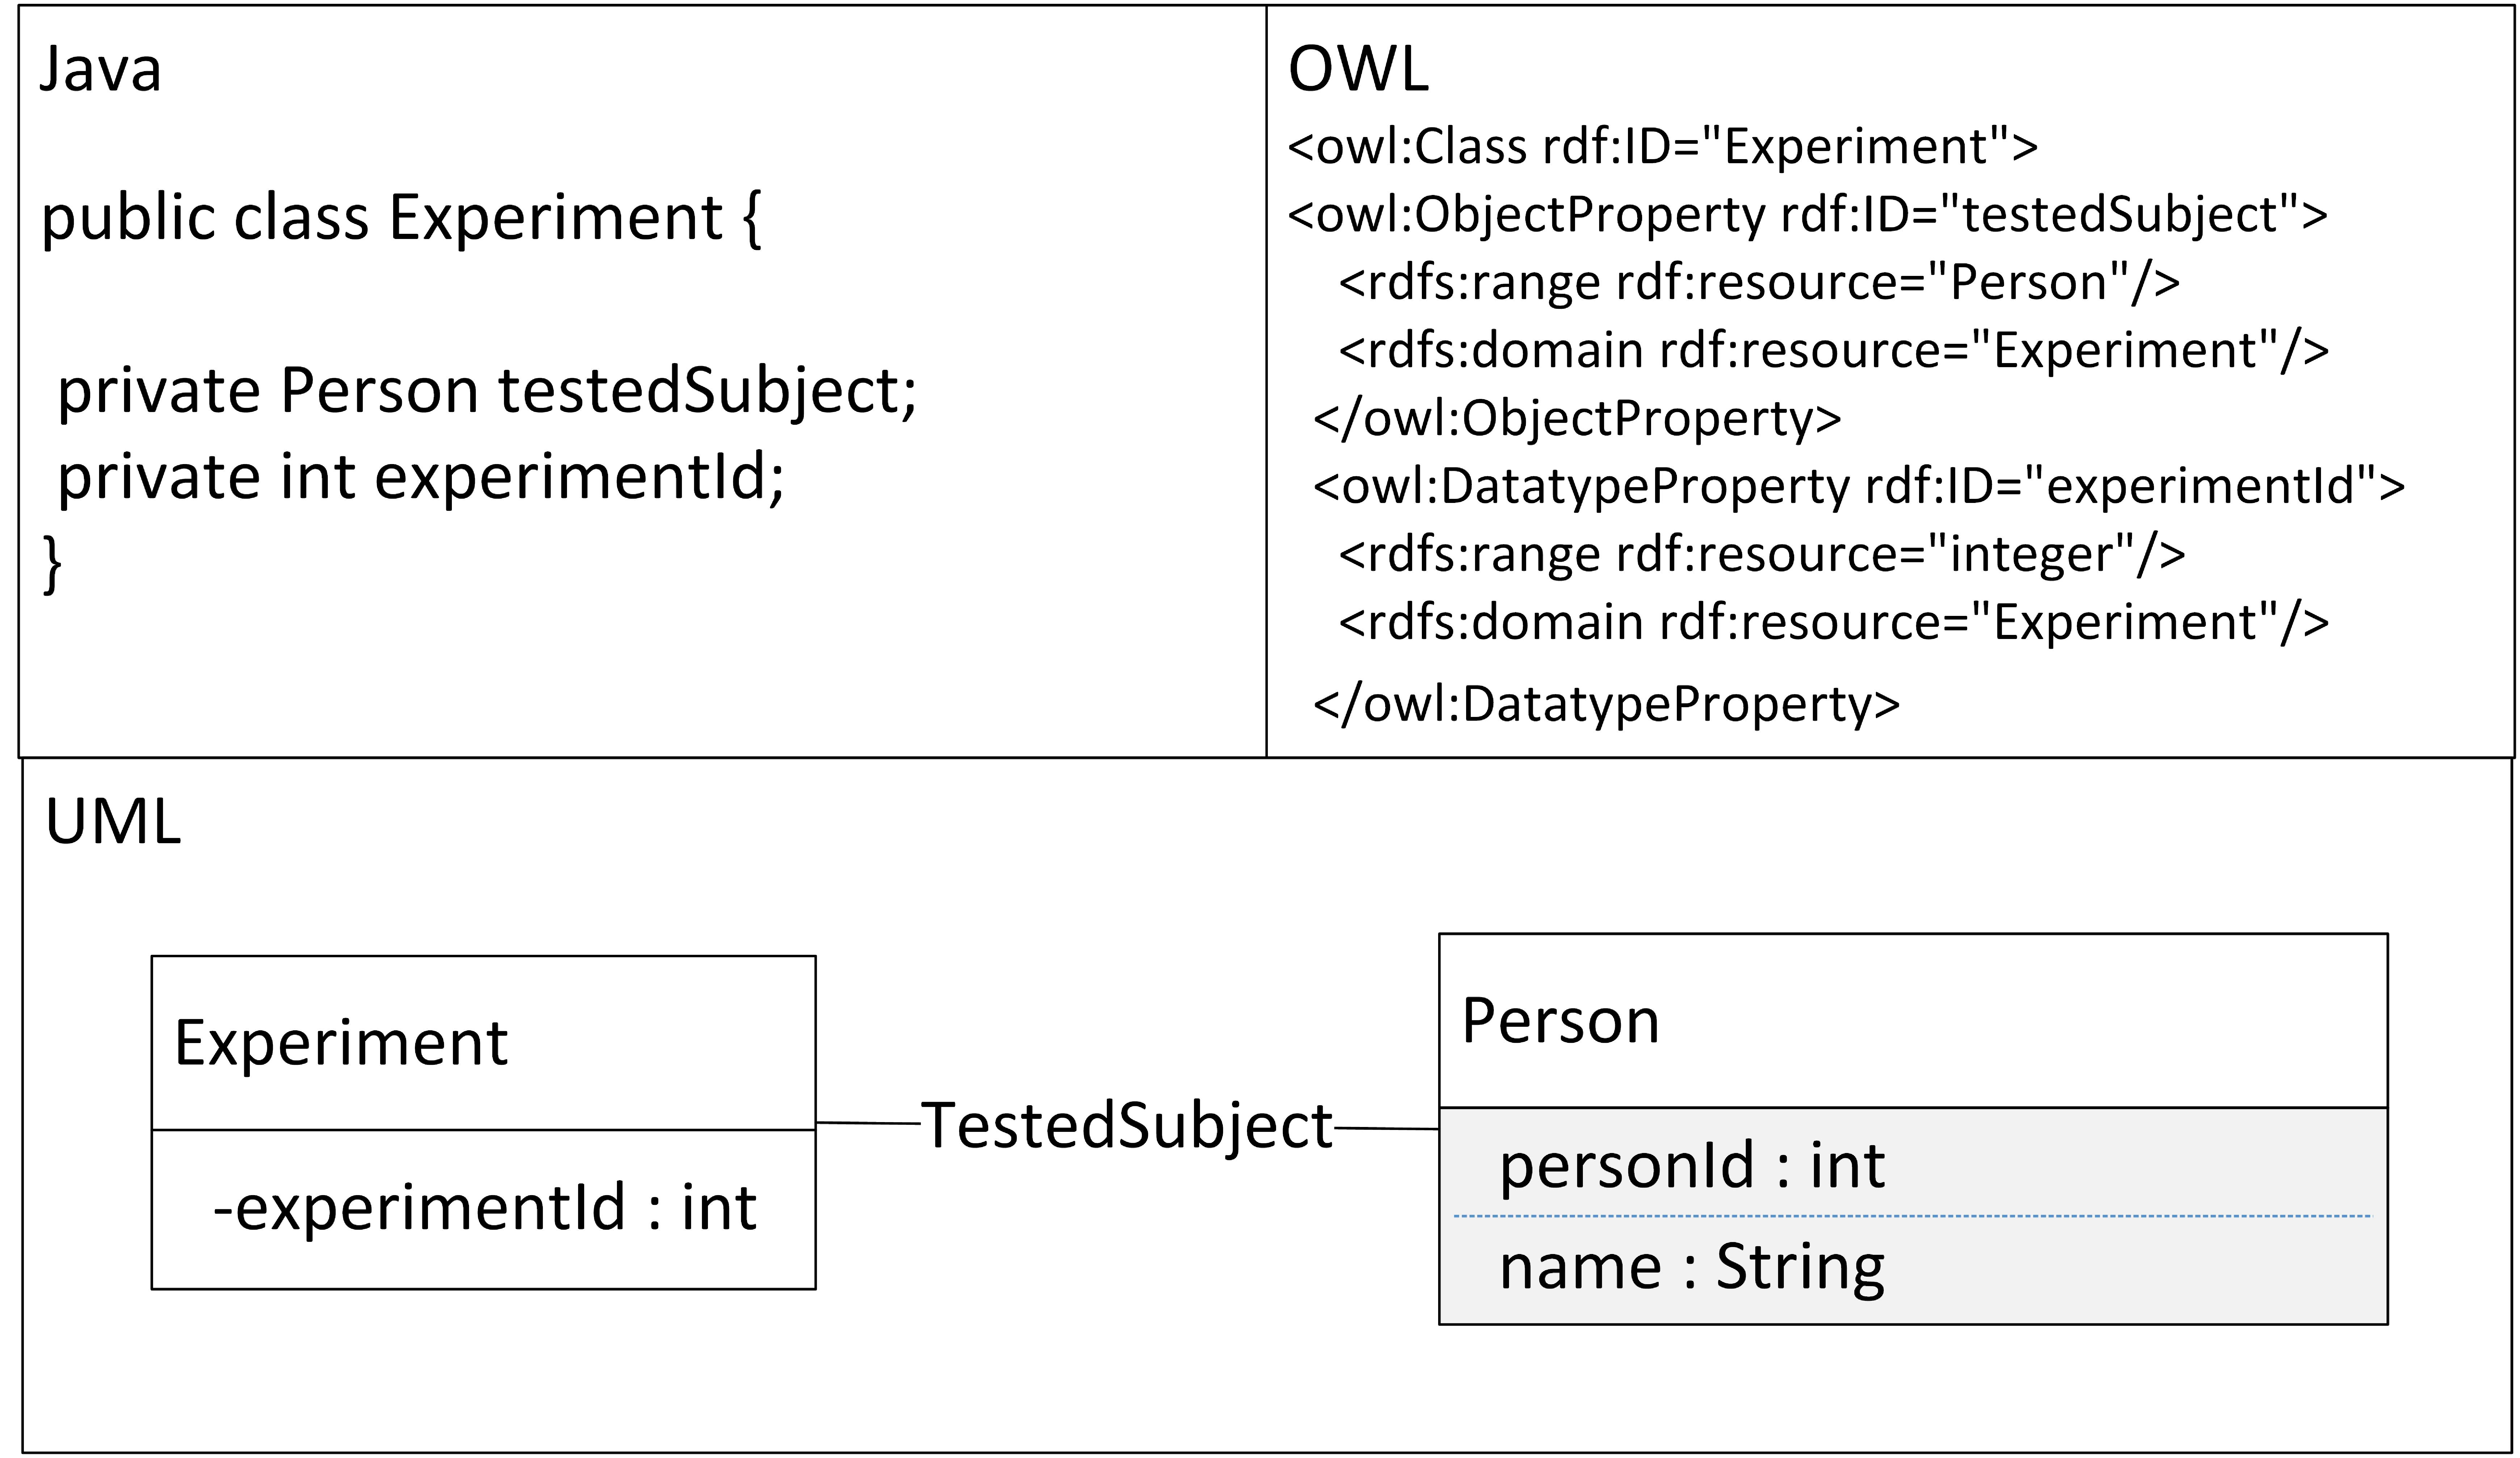
\includegraphics[width = 4.0in]{umlowl1}} \\
\subfloat[Definitions of inheritance and enumeration.]{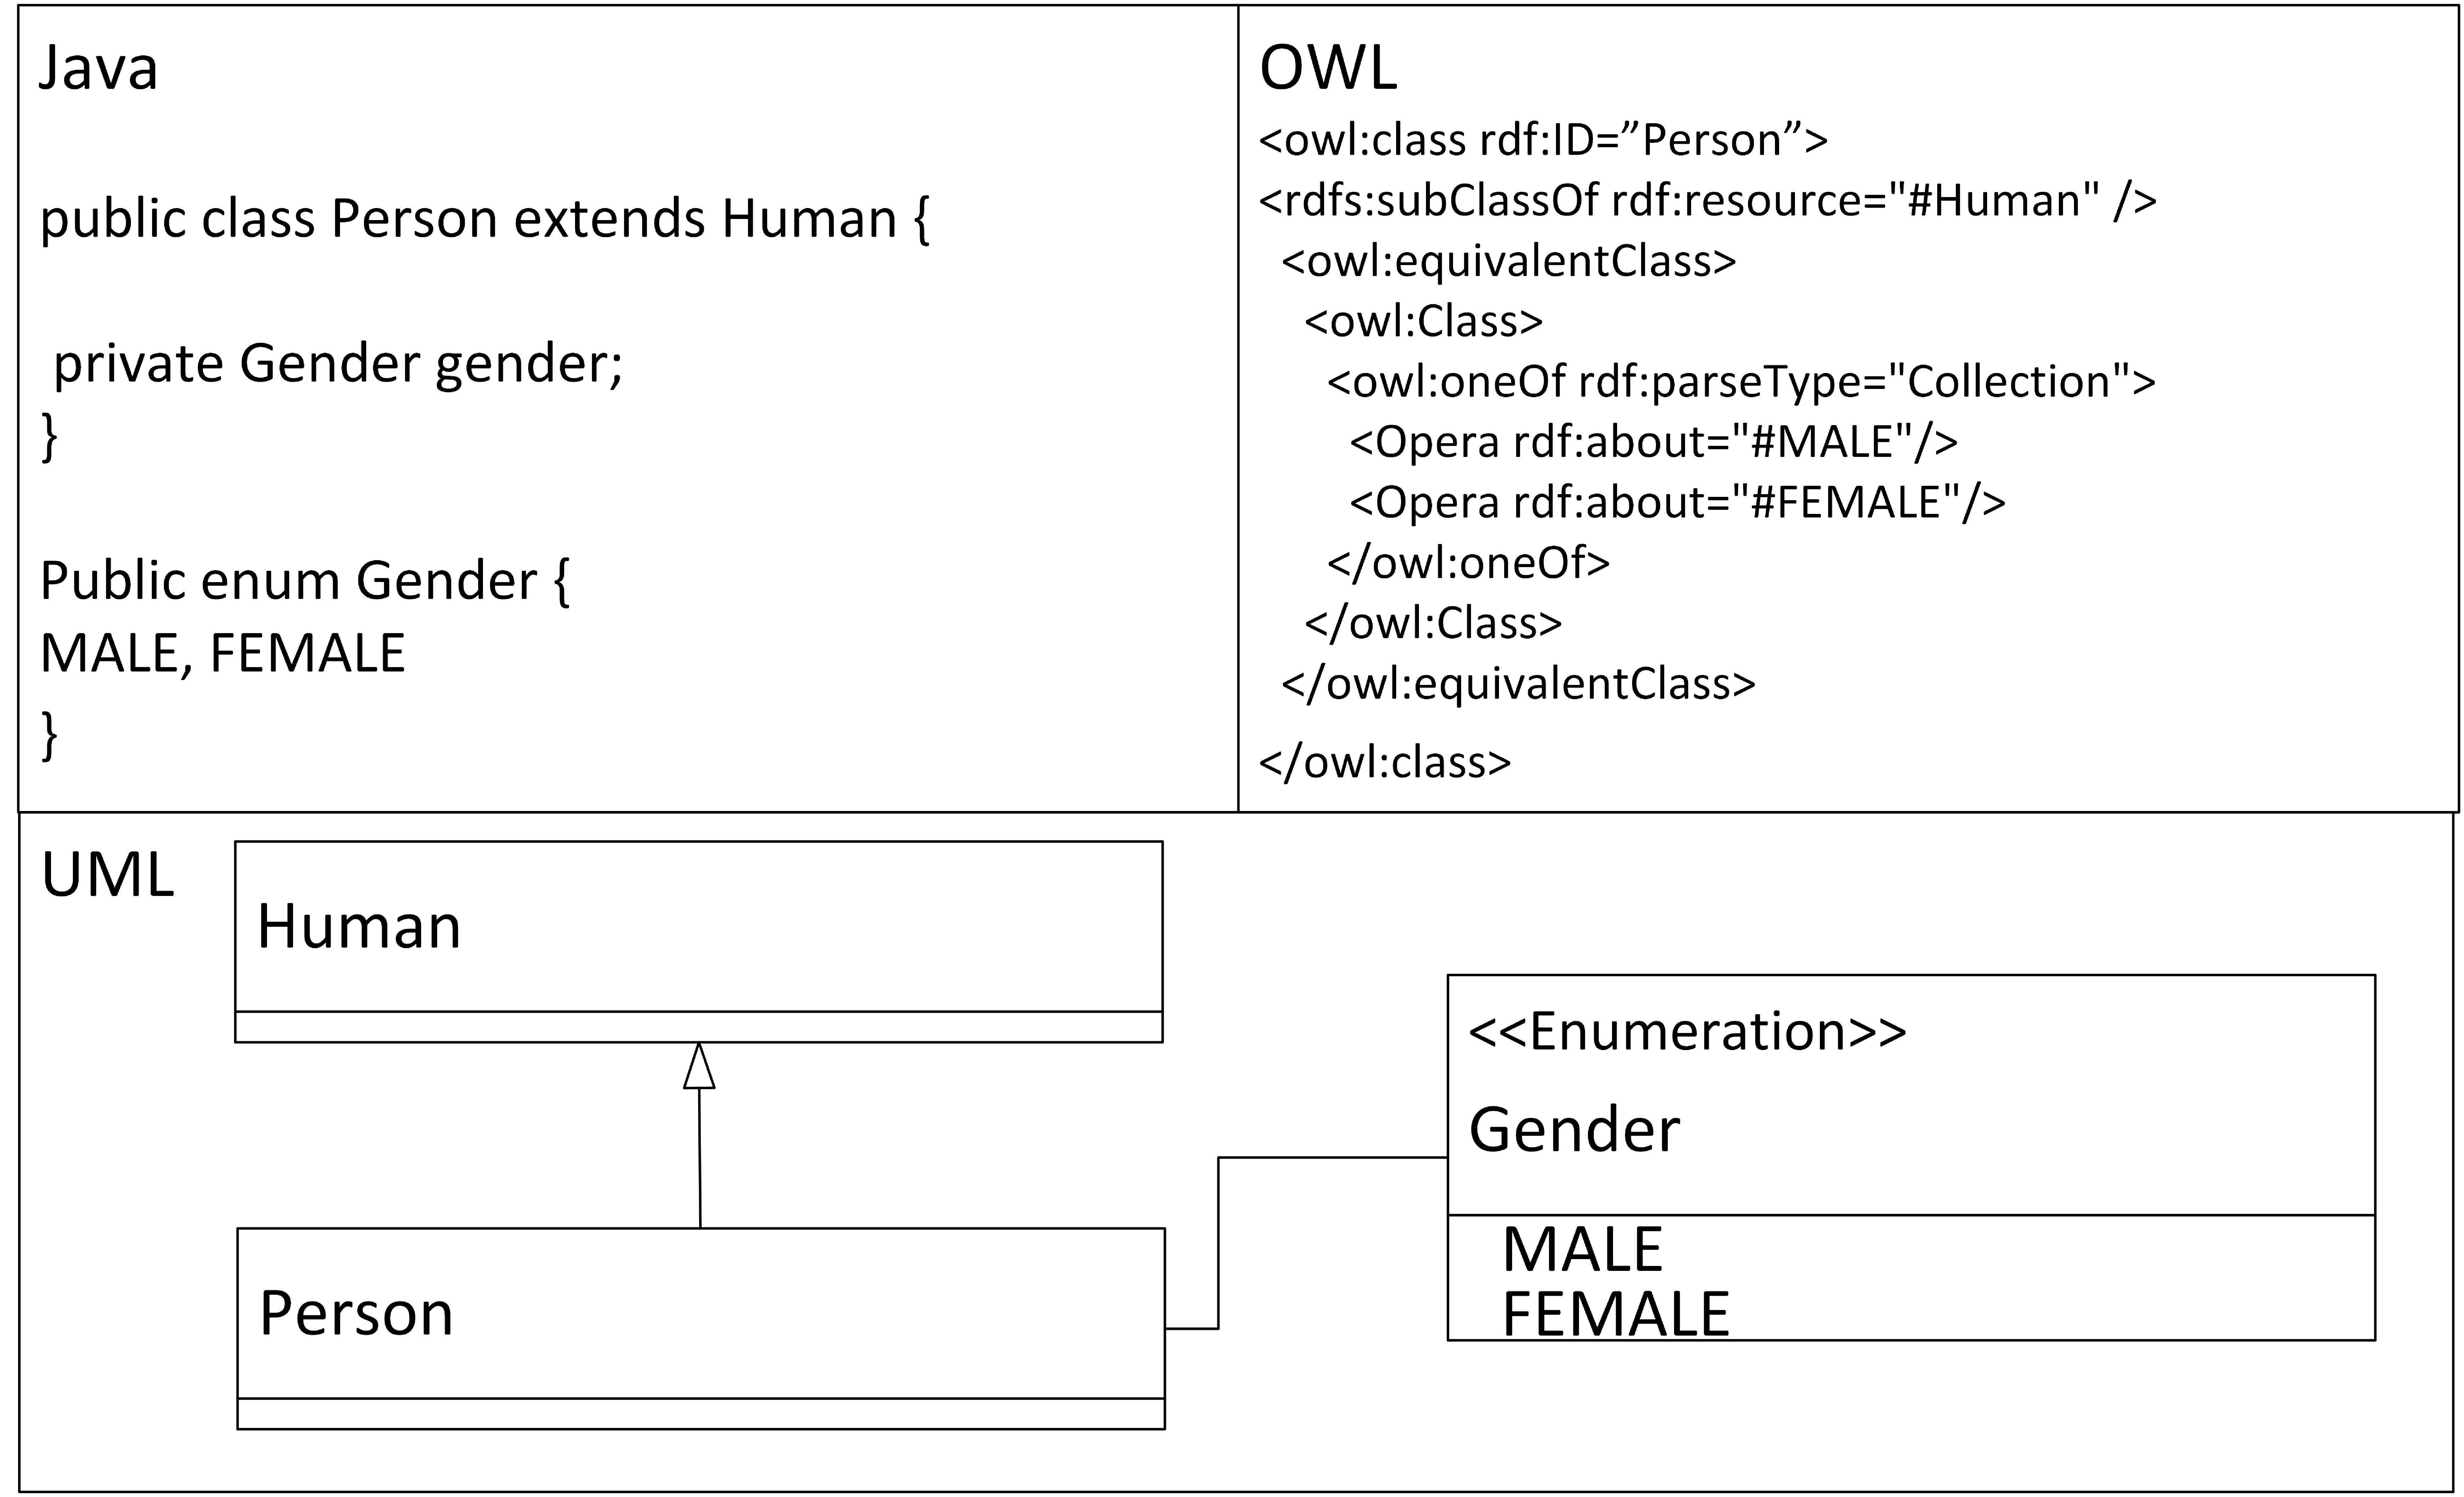
\includegraphics[width = 4.0in]{umlowl2}}  \\
\subfloat[Definitions of disjoint classes.]{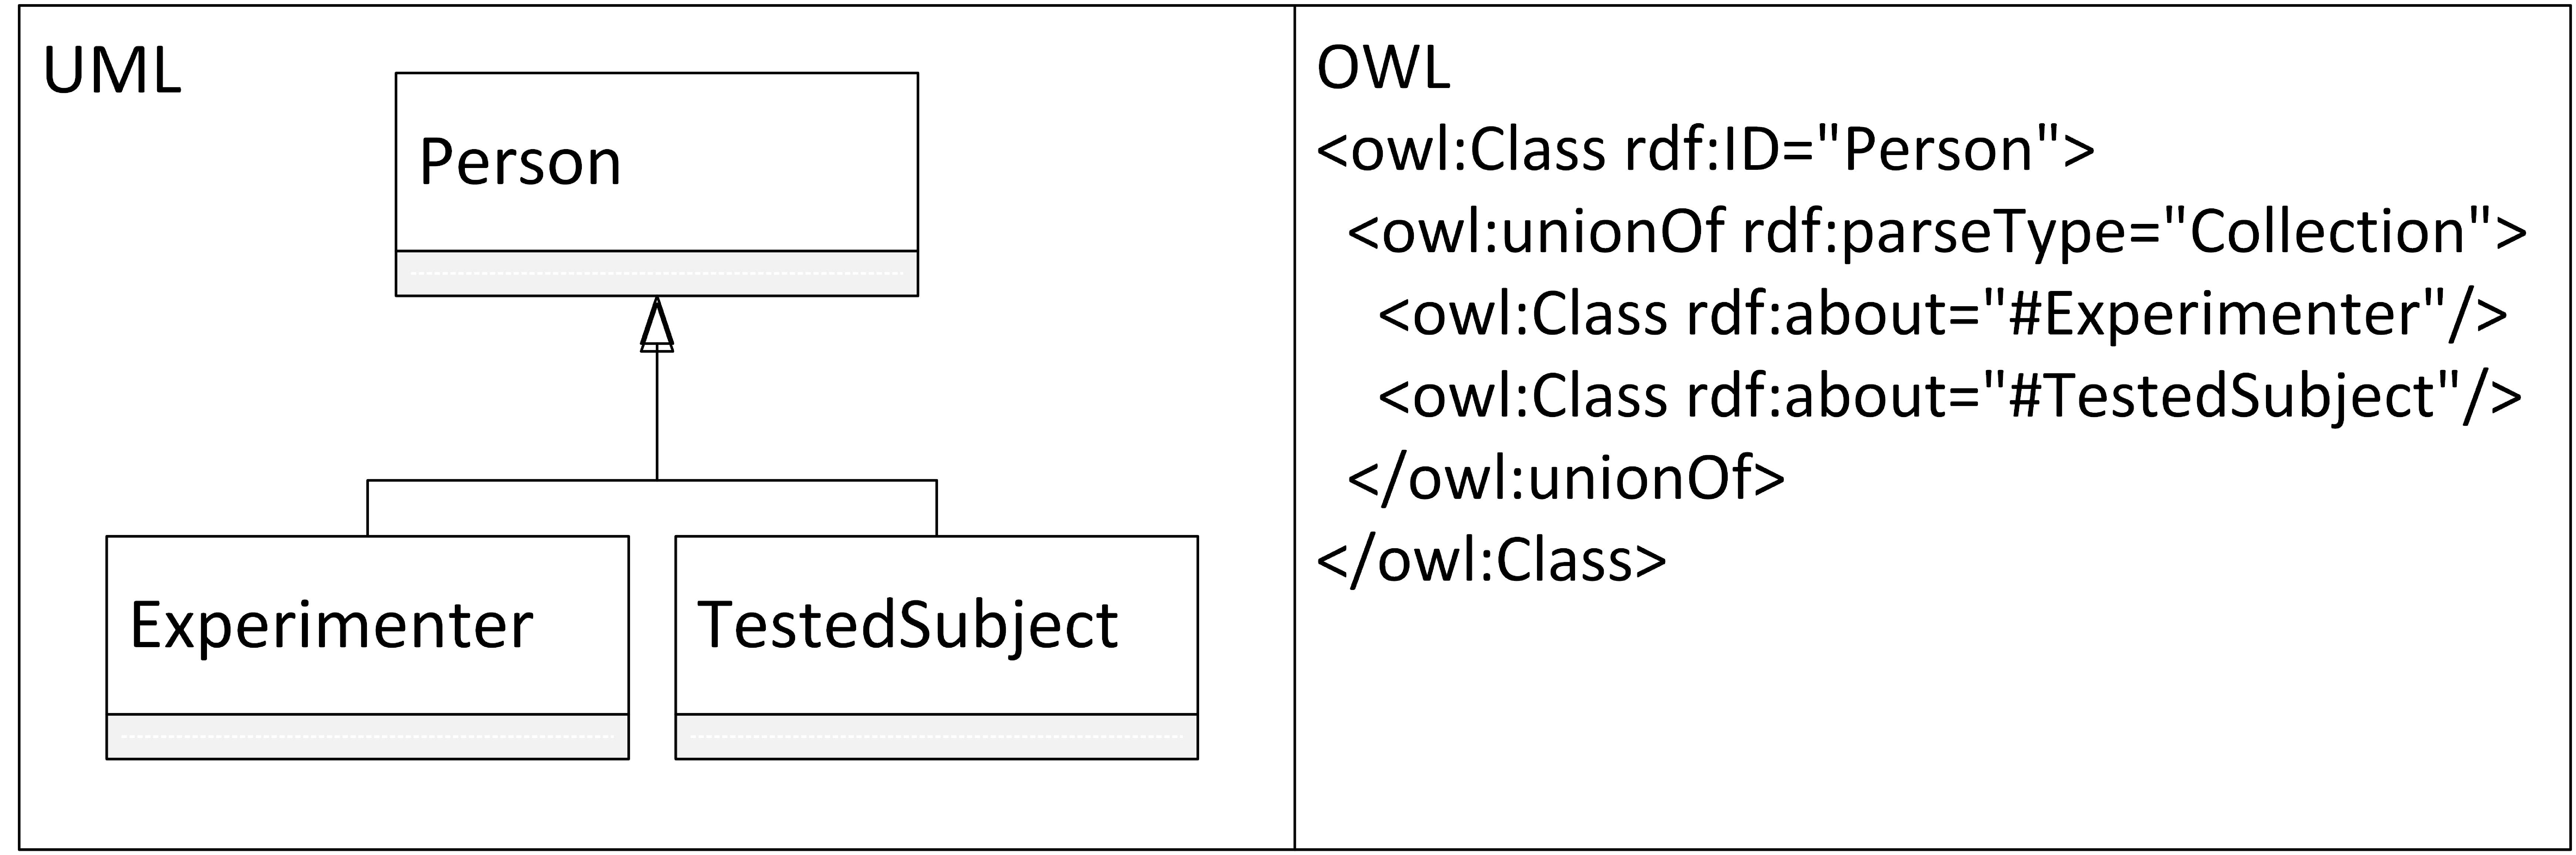
\includegraphics[width = 4.0in]{umlowl3}}
\end{tabular}
% figure caption is below the figure
\caption{Practical Examples of Compared OWL and UML Features.}
\label{fig:umlowlexample}
\end{figure}

\section{Semantic Framework}
\label{Semantic_Framework}

\subsection{Construction of Ontology}
\label{Construction-of-ontology}

According to differences in semantic expressivity described in Section \ref{concepts_comparison}, we propose a custom approach that transforms a common object-oriented syntax to an OWL syntax. The proposed solution is usable by software engineers and not only by experts in the Semantic Web field. Thus, a framework based on common programming technologies is preferred.

Such a solution could serve a wide community of researchers that use object-oriented systems and need to generate ontology. To support this idea, we decided to use only the standard syntactic structures of a commonly used programming language.

Java stores data in JavaBeans\footnote{JavaBeans, as reusable components, are named Java classes with class attributes which
are accessed only by get/set methods.}, often called Plain Old Java Object (POJO). Transformation of a JavaBean representation into an OWL ontology was proved theoretically in Definition \ref{def:JavaBean structure extraction process}.

\begin{definition}
\label{def:JavaBean structure extraction process}
(JavaBean structure extraction process)

\emph{The process is the transformation of a set of JavaBeans J to an ontology O that satisfies:}

\emph{$\forall$ $J{}_{\text{i}}$ $\exists$ OWL class $OC{}_{\text{i}}$ $\in$ O}.

\emph{$\forall$  $J{}_{\text{j}}$ is a superclass of $J{}_{\text{i}}$ $\exists$ OWL class $OC{}_{\text{j}}$ is a superclass of OWL class $OC{}_{\text{i}}$  $\in$  O}.

\emph{$\forall$ field $\in$ $Jf{}_{\text{i}}$ $\exists$  class $OC{}_{\text{i}}$ $\in$  O; its extent is a DataType property $\in$  O $\Leftrightarrow$ $Jf{}_{\text{i}}$ extent is an atomic type}.

\emph{$\forall$ field $\in$ $Jf{}_{\text{i}}$ $\exists$  class $OC{}_{\text{i}}$ $\in$ O; its extent is an Object property $\Leftrightarrow$ $Jf{}_{\text{i}}$ extent is a class $\in$ $J{}_{\text{i}}$}.

\emph{$\forall$ instance of  $J{}_{\text{i}}$ $\bigwedge$ $\forall$ field $Jf{}_{\text{ij}}$  $\exists$ OWL literal $OL{}_{\text{ij}}$ $\in$ O $\hat{=}$ field $\in$ $Jf{}_{\text{ij}}$}.

\end{definition}


\subsection{Proposed Mapping}
\label{Proposed_Mapping}

To give Definition \ref{def:JavaBean structure extraction process} practical sense, an example of Java class mapping to an OWL construct is demonstrated.

An example of a Java object \emph{Experiment} with two attributes, \emph{testedSubject} and \emph{experimentId}, is presented in Listing \ref{Java_class_property_Definition}. The first one is an association relation to the \emph{Person} class, while the second one is an atomic type. Get/set methods are omitted to keep readability. Listing \ref{OWL_individual_Instance} shows a fundamental serialization of this class into an OWL structure. When a sample instance of a described class with assigned sample values \emph{testedSubject=John Smith} and \emph{experimentId=21} is created, its representation is transformed to an \emph{OWL individual}. Serialization of \emph{DataTypeProperty} is straightforward. The property value is directly serialized. Serialization of \emph{ObjectProperty} is solved by serializing an object id value or placing a link that points to the data in the case of binary files.

\begin{lstlisting}[label=Java_class_property_Definition,caption=Java Class Property Definition]
package cz.zcu.kiv;

public class Experiment {

 private Person testedSubject;
 private int experimentId;
}

\end{lstlisting}


\begin{lstlisting}[label=OWL_individual_Instance,caption=OWL Individual Instance]

<cz.zcu.kiv:Experiment rdf:about=
  "http://cz.zcu.kiv#Experiment_21">
  <cz.zcu.kiv:testedSubject>
    <cz.zcu.kiv:Person rdf:about=
      "http://cz.zcu.kiv#Person_511991">
      <cz.zcu.kiv:name rdf:datatype=
        "http://www.w3.org/2001/XMLSchema#string">
        John Smith
      </j.1:name>
    </cz.zcu.kiv:Person>
  </cz.zcu.kiv:testedSubject>
  <cz.zcu.kiv:experimentId rdf:datatype=
    "http://www.w3.org/2001/XMLSchema#int">
    21
  </cz.zcu.kiv:experimentId>
</cz.zcu.kiv:Experiment>
\end{lstlisting}

Although the described mapping works quite satisfactorily, different concepts described in Section \ref{concepts_comparison} are still not covered. When we want to use more capabilities of OWL, we have to enrich the object-oriented code with missing semantics. When we were looking for a suitable way to extend a current object-oriented code, we decided to extend a proposed preliminary idea \citep{conf/iceis/JezekM11} based on using Java Annotations \citep{JavaTutorialAnnotations}.

Java Annotations have several benefits. Firstly, they are a special form of syntactic metadata and can be added to a Java source code. Secondly, they are reflective, i. e. they can be embedded within the compiled code and retrieved at runtime. Thus, we can directly execute a compiled code in the transformation input. Moreover, Java Annotations are a part of the Standard Java Development Kit; since Java 5.0, they can be processed immediately. Finally, Java Annotations are used in current software development (by several common frameworks, e.g. Spring, Hibernate, Java Persistent API); hence, software developers can work with this extension without difficulties. Such a JavaBean extension can be immediately used by software engineers. It does not matter if they are familiar with the development of the Semantic Web or not.

The theoretical extraction of JavaBeans annotations and its transformation to OWL documents is formally described in Definition \ref{def:Java_annotation_extraction_process}.

\begin{definition}
\label{def:Java_annotation_extraction_process}
(Java annotation extraction process)

\emph{The process is the transformation of a set of Java annotations JA to a resources R  in the ontology O that satisfies:}

\emph{$\forall$ $JA{}_{\text{i}}$ $\exists$ OWL class $R{}_{\text{i}}$ $\in$ O $\Rightarrow$ $JA{}_{\text{i}}$ $\in$ a class annotation}.

\emph{$\forall$ $JA{}_{\text{i}}$ $\exists$ OWL property $R{}_{\text{i}}$ $\in$ O $\Rightarrow$ $JA{}_{\text{i}}$ $\in$ a property annotation}.

\end{definition}

A practical realization is demonstrated in Listing \ref{Annotated_Java_Bean_Example}. The class Person is presented again with an attribute testedPerson as defined in Listing \ref{Java_class_property_Definition}. The example demonstrates usage of two annotations. The first one defines an \emph{equivalent class} to the Experiment class. The second one shows the definition of an \emph{equivalent property} of the testedSubject property. The serialization of such a JavaBean is shown in Listing \ref{Annotated_Java_Bean_OWL_Serialization}.

\begin{lstlisting}[label=Annotated_Java_Bean_Example,caption=Annotated Java Bean Example]
package cz.zcu.kiv;

@EquivalentClass
  ("http://cz.zcu.kiv/Measurement")
public class Experiment {

  @EquivalentProperty
    ("http://cz.zcu.kiv/TestedSubject")
  private Person testedPerson;
}
\end{lstlisting}


\begin{lstlisting}[label=Annotated_Java_Bean_OWL_Serialization,caption=Annotated Java Bean OWL Serialization, escapechar=@]
<owl:Class rdf:about=
  "http://cz.zcu.kiv/Measurement"/>
<owl:Class rdf:about=
  "http://cz.zcu.kiv#Experiment">
 @\textbf{
 $<$owl:equivalentClass rdf:resource= }@
 @\textbf{    "http://cz.zcu.kiv/Measurement"/$>$
    }@
</owl:Clas>
<owl:ObjectProperty rdf:about=
  "http://cz.zcu.kiv#testedPerson">
@\textbf{
  $<$owl:equivalentProperty rdf:resource=  }@
@\textbf{    "http://cz.zcu.kiv/TestedSubject"/$>$
  }@
  <rdfs:domain rdf:resource=
   "http://cz.zcu.kiv#Experiment"/>
</owl:ObjectProperty>
\end{lstlisting}

We have selected the concepts that have a class and/or property extent \citep{BMEI_jezek_moucek}. According to the different concepts types described in Section \ref{concepts_comparison} we have defined a set of annotations described in Table \ref{tab:Java annotations to OWL mapping}. The table specifies currently defined annotations and their mapping to the OWL constructs. Most designed annotations are parameterizable. Parameter values shown in Table \ref{tab:Java annotations to OWL mapping} are demonstration examples; they can be changed according to the needs of a specific domain. The set of supported annotations is continually extended. New annotations are gradually proposed and implemented.

\begin{table}

\centering
\footnotesize
\renewcommand{\arraystretch}{1}
\tabcolsep=0.11cm
\catcode`\-=12
\caption{\label{tab:Java annotations to OWL mapping}OWL Mapping of Java Annotations}
\begin{tabular}{ll}

\hline
\textbf{Java Annotation} & \textbf{OWL construct}
\tabularnewline
\hline
@EquivalentClass & $<$owl:equivalentClass rdf:resource=\\
("http://www.kiv.zcu.cz/Person") & \hspace{3mm}"http://www.kiv.zcu.cz/Person"/$>$
\tabularnewline
\hline
@EquivalentProperty & $<$owl:equivalentProperty rdf:resource=\\
("http://www.kiv.zcu.cz/first\_name") &\hspace{3mm}"http://www.kiv.zcu.cz/first\_name"/$>$ \\

\hline
@Symmetric & $<$rdf:type rdf:resource="http:/www.w3.org\\
& /2002/07/owl\#SymmetricProperty"/$>$ \\
\hline
@Inverse & $<$owl:inverseOf rdf:resource=\\
("http://www.kiv.zcu.cz/givenname") &\hspace{3mm}"http://www.kiv.zcu.cz/givenname"/$>$\\

\hline
@AllValuesFrom & $<$owl:allValuesFrom rdf:resource=\\
("http://www.kiv.zcu.cz/\#Persons") &\hspace{3mm}"http://www.kiv.zcu.cz/\#Persons"/$>$ \\
\hline
@Transitive& $<$rdf:type rdf:resource=\\
 &\hspace{3mm}"http://www.w3.org/2002/07/owl\\
& \#TransitiveProperty"/$>$ \\
\hline
@AllDifferent & $<$rdf:type rdf:resource=\\
("http://www.kiv.zcu/Experiment") & \hspace{3mm}"http://www.kiv.zcu.cz/\#AllDifferent"/$>$\\
\hline
@DifferentFrom & $<$owl:differentFrom rdf:resource=\\
("http://www.kiv.zcu.cz/Experiment") & \hspace{3mm}"http://www.kiv.zcu/Experiment"/$>$ \\
\hline
@SameAs & $<$owl:sameAs rdf:resource=\\
("http://www.kiv.zcu.cz/Experiment") & \hspace{3mm}"http://www.kiv.zcu/Experiment"/$>$ \\
\hline
@Cardinality(1) &         $<$owl:cardinality rdf:datatype=\\
&\hspace{3mm}"http://www.w3.org/2001/XMLSchema\\
&\hspace{3mm}\#int"$>$1$<$/owl:cardinality$>$\\
\hline
@MaxCardinality(1) & $<$owl:maxCardinality rdf:datatype\\
&\hspace{3mm}="http://www.w3.org/2001/XMLSchema\\
&\hspace{3mm}\#int"$>$1$<$/owl:maxCardinality$>$\\

\hline
@MinCardinality(1) & $<$owl:minCardinality rdf:datatype\\
&\hspace{3mm}="http://www.w3.org/2001/XMLSchema\\
&\hspace{3mm}\#int"$>$1$<$/owl:minCardinality$>$\\

\hline
@SomeValuesFrom & $<$owl:someValuesFrom rdf:resource=\\
 ("http://www.kiv.zcu/Person") & \hspace{3mm} "http://www.kiv.zcu/Person"/$>$\\
\hline

\end{tabular}


\end{table}

\subsection{Implementation}
\label{Implementation}

The described mapping resulted in a practical implementation in a proprietary solution called the Semantic Framework. It is a library with the input in the form of the set of JavaBeans and the output in the form of an ontology document. We did not implement the Semantic Framework  from scratch but it is based on the existing tools that we modified.  The core of the system is modified JenaBean \citep{citeulike:JenaBean}. JenaBean internally uses the Jena Framework \citep{morningboat:jena16} that is responsible for creation of an internal semantic model.


Figure \ref{fig:Semantic_Framework} shows the component diagram of the Semantic Framework. The first subcomponent is the modified JenaBean. The \emph{Extended JenaBean} enables transformation of the output to correspond with the described mapping. Moreover, the processing of Java annotations was added. The output of the \emph{Extended JenaBean} component is an internal model representation. This internal model representation is submitted to the second, \emph{Ontology Model Creator}, subcomponent. This subcomponent creates an Ontology model using an \emph{Ontology Model Factory}. The internal JenaBean model is processed and an ontology document is created by calling Jena API methods. The resulting model can be further processed by the last subcomponent, \emph{OWL API} \citep{DBLP:journals/semweb/HorridgeB11}, which is able to transform an ontology model into supported ontology formats. The UML diagram describing the usage of the Semantic Framework is in Figure \ref{fig:Semantic_Framework_class_diagram}.

\begin{figure}
% Use the relevant command to insert your figure file.
% For example, with the graphicx package use
  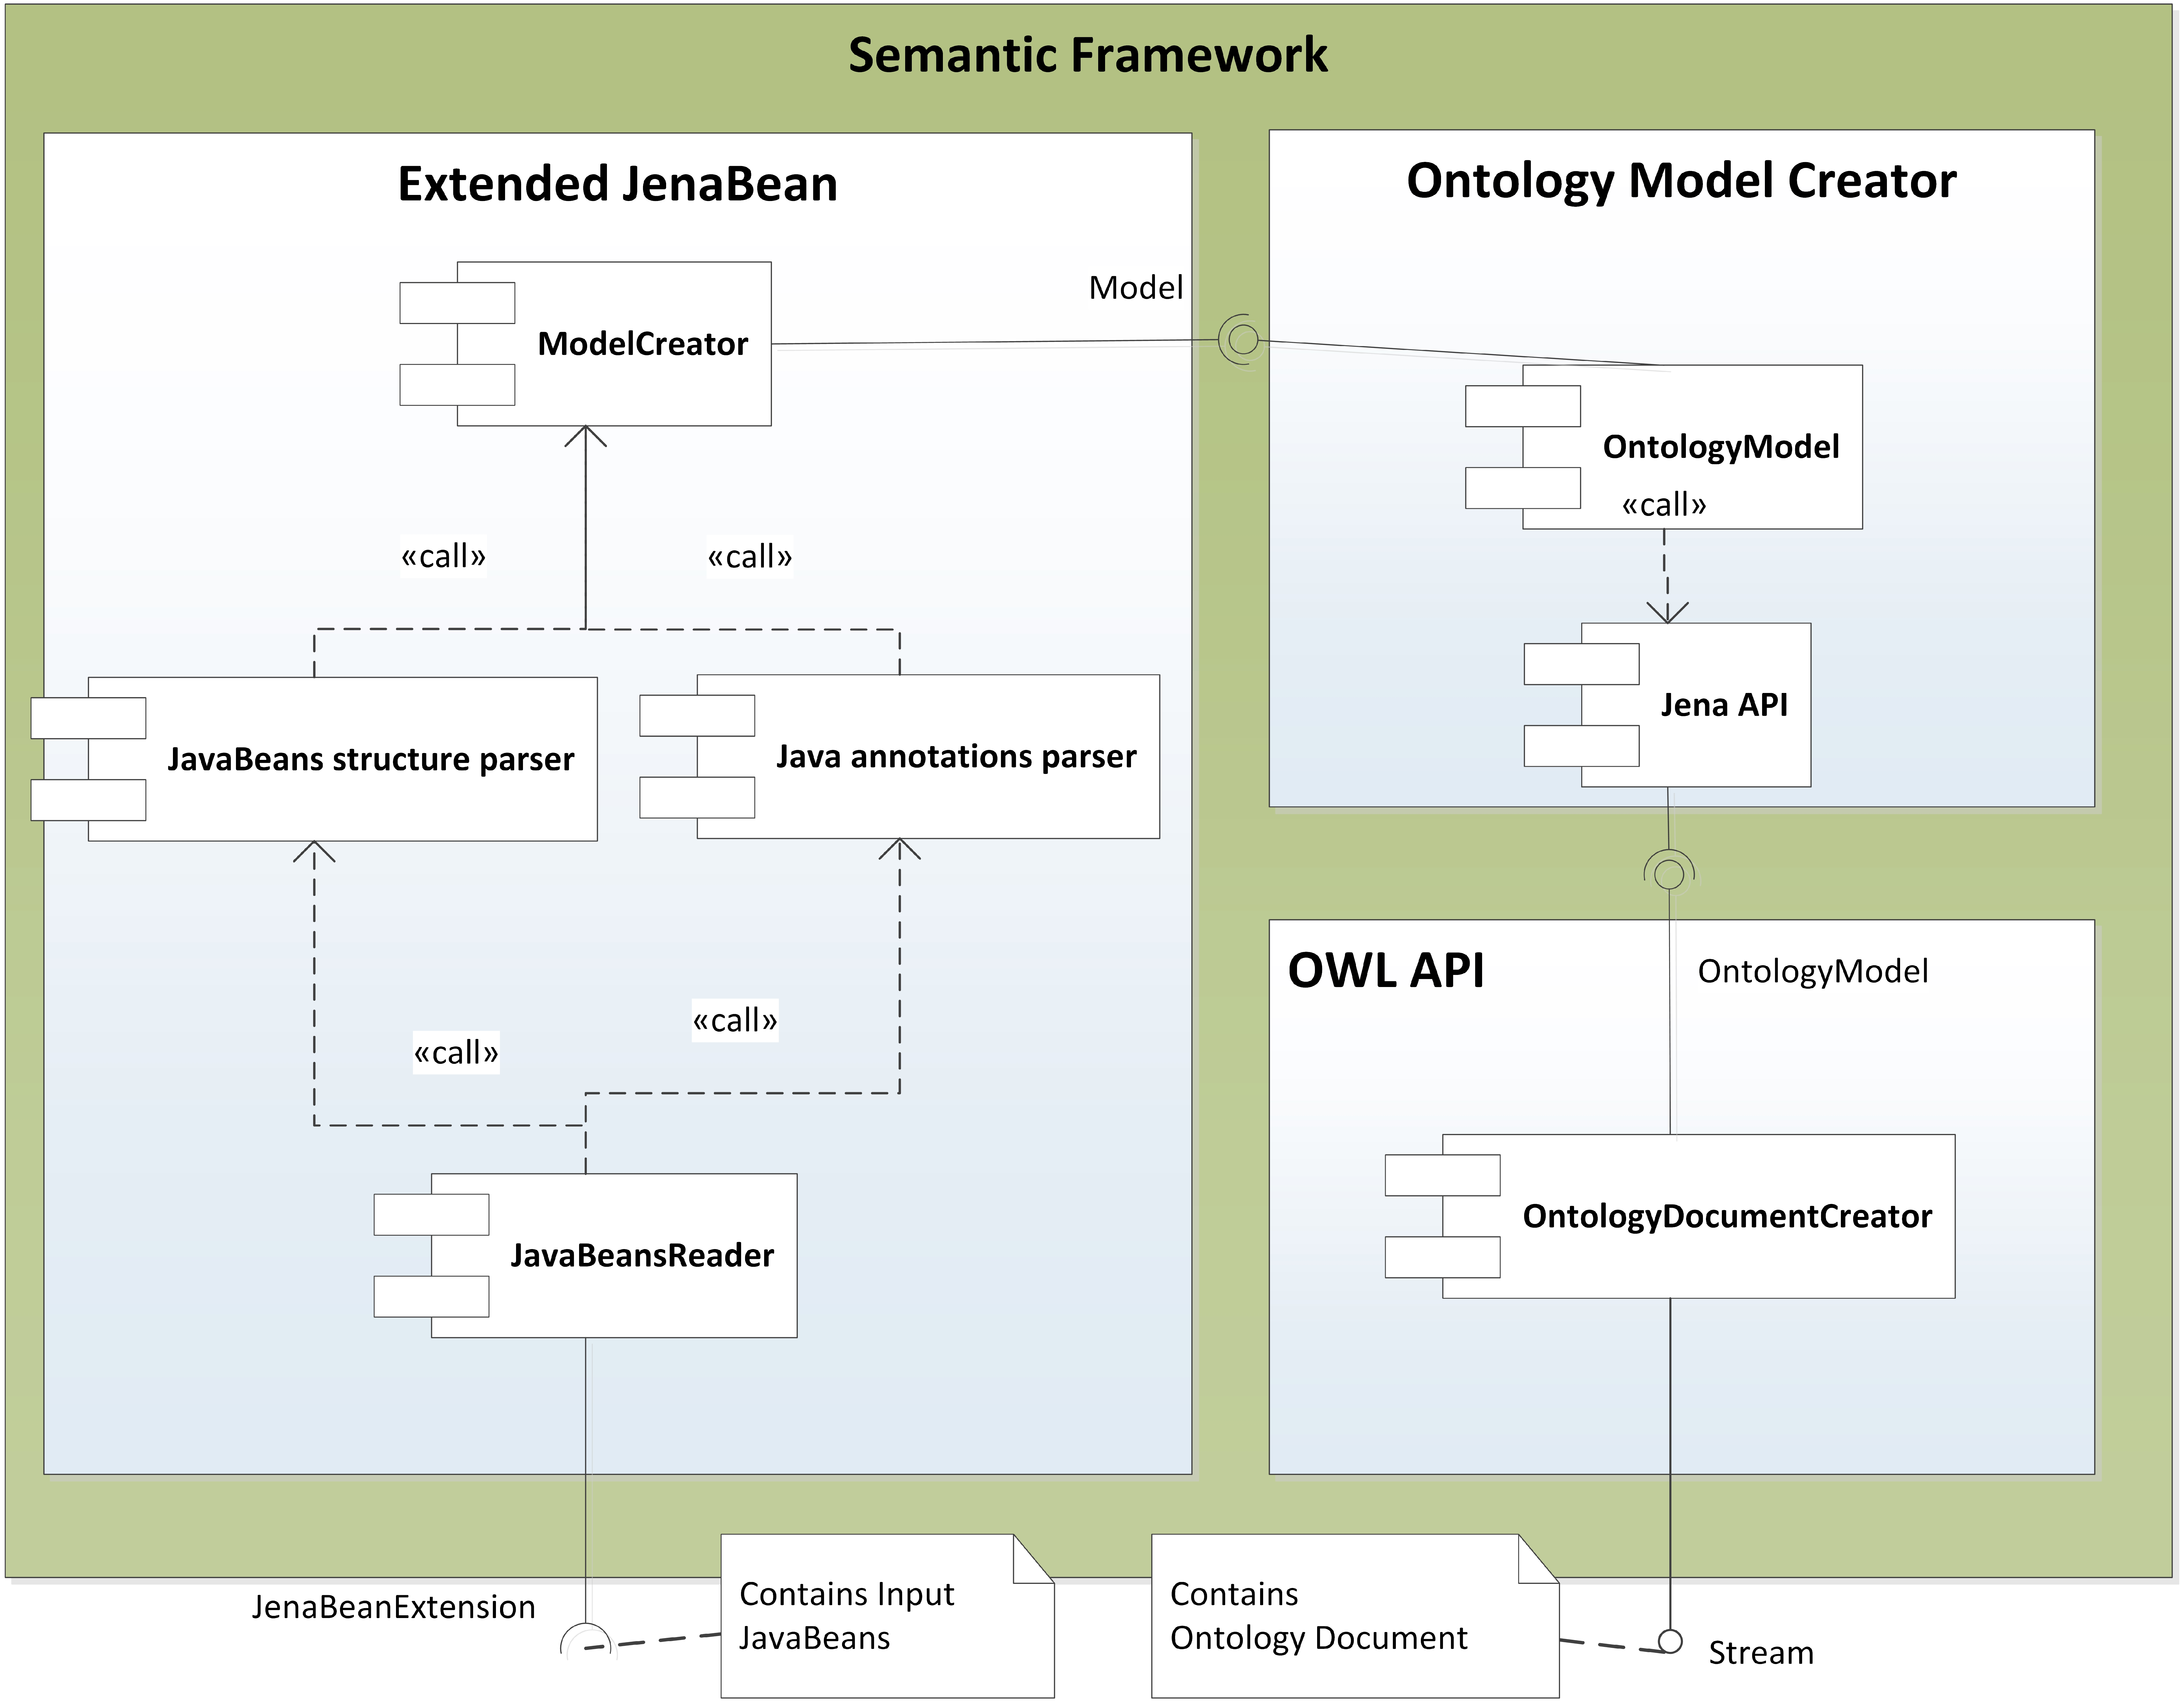
\includegraphics[width=15cm]{SemanticFramework_Component_Model}
% figure caption is below the figure
\caption{Component Diagram of Semantic Framework. The Semantic Framework reads a list of input JavaBeans using an implemented reader based on Java Reflection API \citep{jlfalcone:sun:06}. This list passes through two parsers. The first one reads a JenaBean structure; the second one reads supplemented annotations. The parsers create an internal representation. Such a representation is read by Jena API, which provides a model suitable for an OWL API. The OWL API implements existing OWL syntaxes and provides methods for serializing the model.}
\label{fig:Semantic_Framework}
\end{figure}



\begin{figure}
\center
% Use the relevant command to insert your figure file.
% For example, with the graphicx package use
  
\includegraphics[width=15cm]{SemanticFramework_uml}
% figure caption is below the figure
\caption{Class Diagram of Semantic Framework Interface. The Actor1 represents a client program. The client calls interface \emph{JenaBeanExtension} with one method, \emph{getOntologyDocument}, that returns ontology document in a \emph{Stream}. The returned stream can be serialized into supported formats by an \emph{OwlApi} interface calling a \emph{convertToSemanticStandard} method. }
\label{fig:Semantic_Framework_class_diagram}
\end{figure}


\section{Performance Evaluation}
\label{Performance_evaluation}

\subsection{Experimental Verification}
\label{Experimental_Verification}

We discuss the complexity of the algorithm in a practical scenario. Firstly, we prepared a set of \emph{Experiment} instances. Then, we assigned instances of \emph{Person}, \emph{Scenario}, \emph{Hardware} and \emph{Data} to each experiment. The class \emph{Person} was extended by the set of supported annotations from Table \ref{tab:Java annotations to OWL mapping}. The tests were run ten times and the result was created as an average of partial results.

The chart in Figure \ref{fig:results} shows the linearity of the transformational process.  Tested syntaxes are functionally equivalent; they differ only in the format of the serialized output document \citep{Wurlitzer:Beckett:04:RSS}.

\begin{figure}
  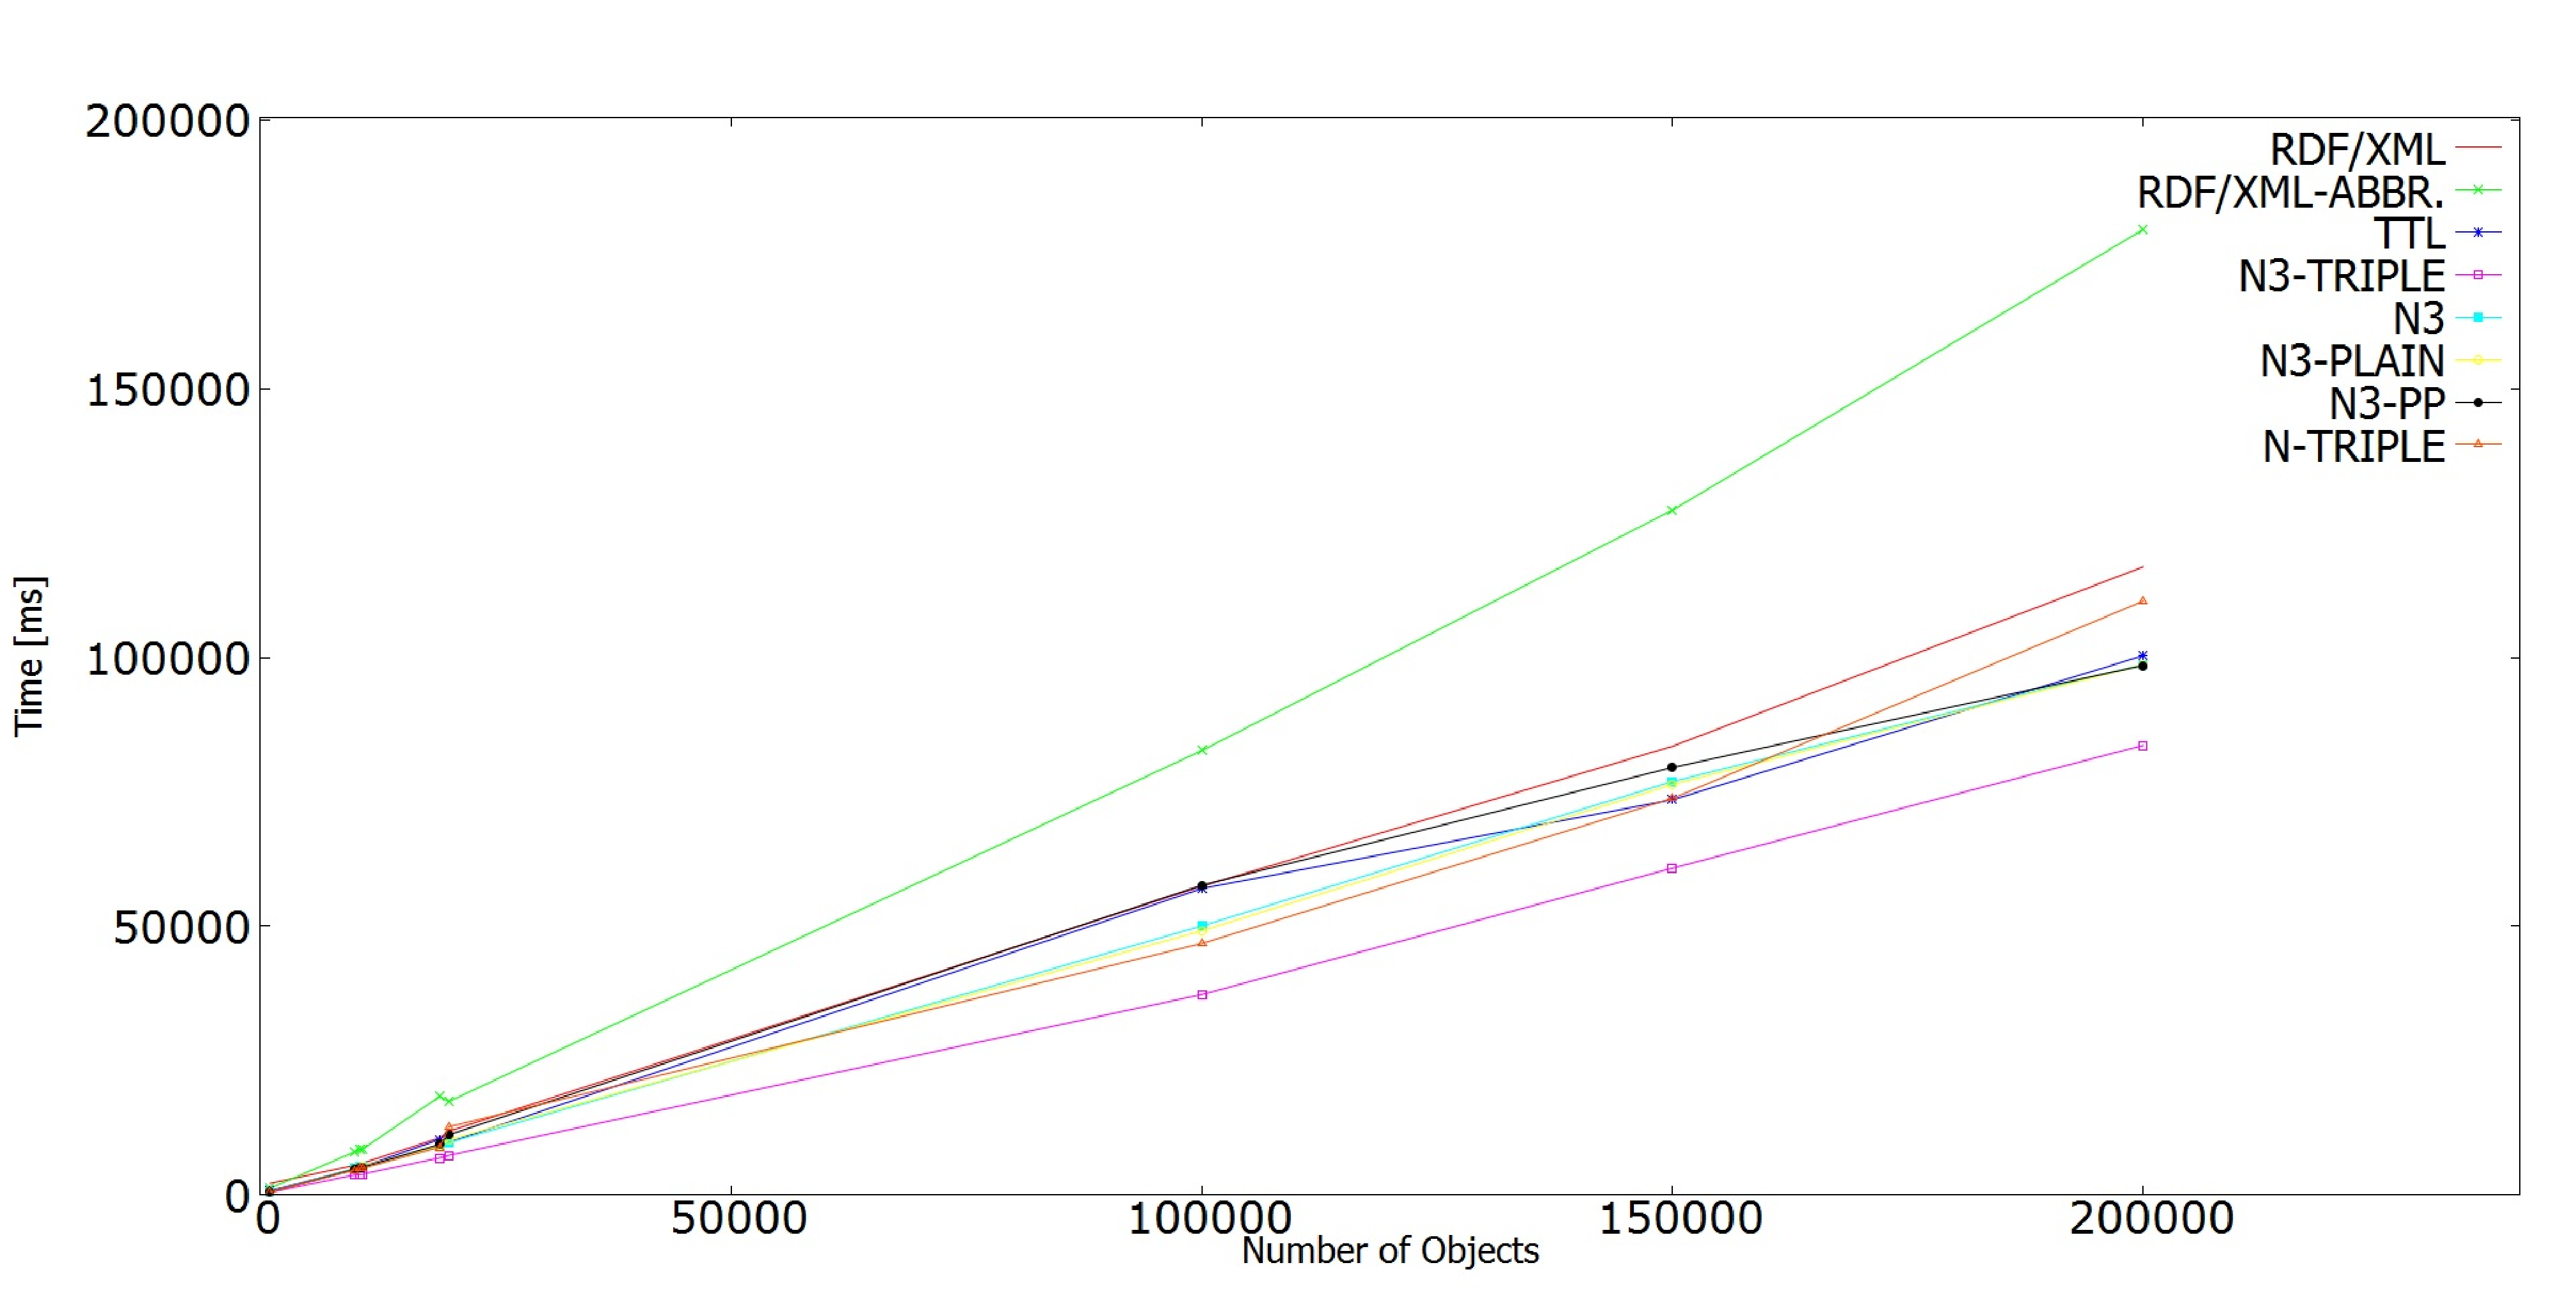
\includegraphics[width=18cm]{result}
% figure caption is below the figure
\caption{Time Dependence of Transformation on the Number of Objects for Supported Syntaxes. The time dependence is fundamentally linear for each syntax. Practically, this means that the transformation is directly dependent only on the number of input objects.}
\label{fig:results}
\end{figure}


\section{Experimental Evaluation}
\label{discussion}

\subsection{Experimental Ontology}
\label{Experimental_Ontology}
As experimental data-sharing initiatives continue to expand within the neurophysiological community, the need for descriptive ontology increases. NEMO \citep{DouFRFMT07} is intended as a complex ontology describing EEG, averaged EEG (ERPs), and ERP data analysis results. Even though NEMO is a completely ontology-based approach, the community still uses tools based on common programming technologies. In addition, NEMO seems to be too complex to be immediately deployed in specific electrophysiology domains. Facing difficulties with management of experiments obtained within our laboratory, we defined a simpler ontology that precisely describes the domain of EEG/ERP experiments. This ontology is based on experience in our laboratory, scientific papers and books describing EEG/ERP experiments (e. g. \citep{luck}). Semantically, it is a modified subset of NEMO.

The internal ontology structure corresponds to metadata items collected during experiments. The collected metadata are divided into several semantic groups. We defined the following semantic groups: Activity, Environment, Tested subject, Hardware equipment, Software equipment, Used electrodes, Data digitalization, Signal analysis, Data presentation, and Signal artifact.

\subsection{Implementation within EEG/ERP Portal}
\label{Implementation-within-EEG-ERP-Portal}

The EEG/ERP Portal \citep{ISI:000306821100004} is intended for experimental data-sharing and management. The internal structure of the EEG/ERP portal is designed respecting INCF recommendations \citep{incf-sustainability-report}. Experimental ontology described in Section \ref{Experimental_Ontology} has been developed within the EEG/ERP Portal. The data layer of the Portal is implemented using a relational database (Oracle 11g) and its persistent layer is represented by POJOs. An object-relational mapping (ORM) is ensured by the Hibernate framework \citep{Bauer:2006:JPH:1212283}. The internal structure of the layer is implemented according to the defined ontology. A user who wants to upload a custom experiment into the system fills out a set of predefined forms with metadata. These metadata are input data for the desired ontology.


\subsection{Semantic Framework Integration with EEG/ERP Portal}
\label{Semantic_Framework_Integration_with_EEG_ERP_Portal}

The EEG/ERP Portal is a tool developed using common programming technologies. If we want to register the EEG/ERP Portal as a recognized data source, we need to transform the internal ontology into the Semantic Web structures. The Semantic Framework developed has been integrated into the EEG/ERP Portal (Figure \ref{fig:Semantic_Framework_Integration_in_EEG_ERP_Portal}). The internal logic\footnote{A Spring MVC is used. It practically implements a Model-View-Controller design pattern.} calls a Semantic Framework API using a built-in timer. This timer calls the Semantic Framework API at regular intervals; the ontology document is stored in a temporary file where this document is immediately available. It ensures a faster response of the system.

\begin{figure}
\center
  
\includegraphics[width=12cm]{EEG_ERP_Portal_Semantic_Framework_Integration}
\caption{Integration of the Semantic Framework in the EEG/ERP Portal. The EEG/ERP Portal is a layered architecture designed according to a Model-View-Controller design pattern. The data layer obtains Javabeans from a relational database. The application layer is controlled by the set of \emph{Controllers} which process user requests originated from a web browser. The specific controller (\emph{Semantic Controller}) processes ontology document requests. This controller calls the integrated Semantic Framework through \emph{Semantic Factory} and returns a serialized ontology document to the user's web browser.}
\label{fig:Semantic_Framework_Integration_in_EEG_ERP_Portal}
\end{figure}





\begin{figure}
\center
  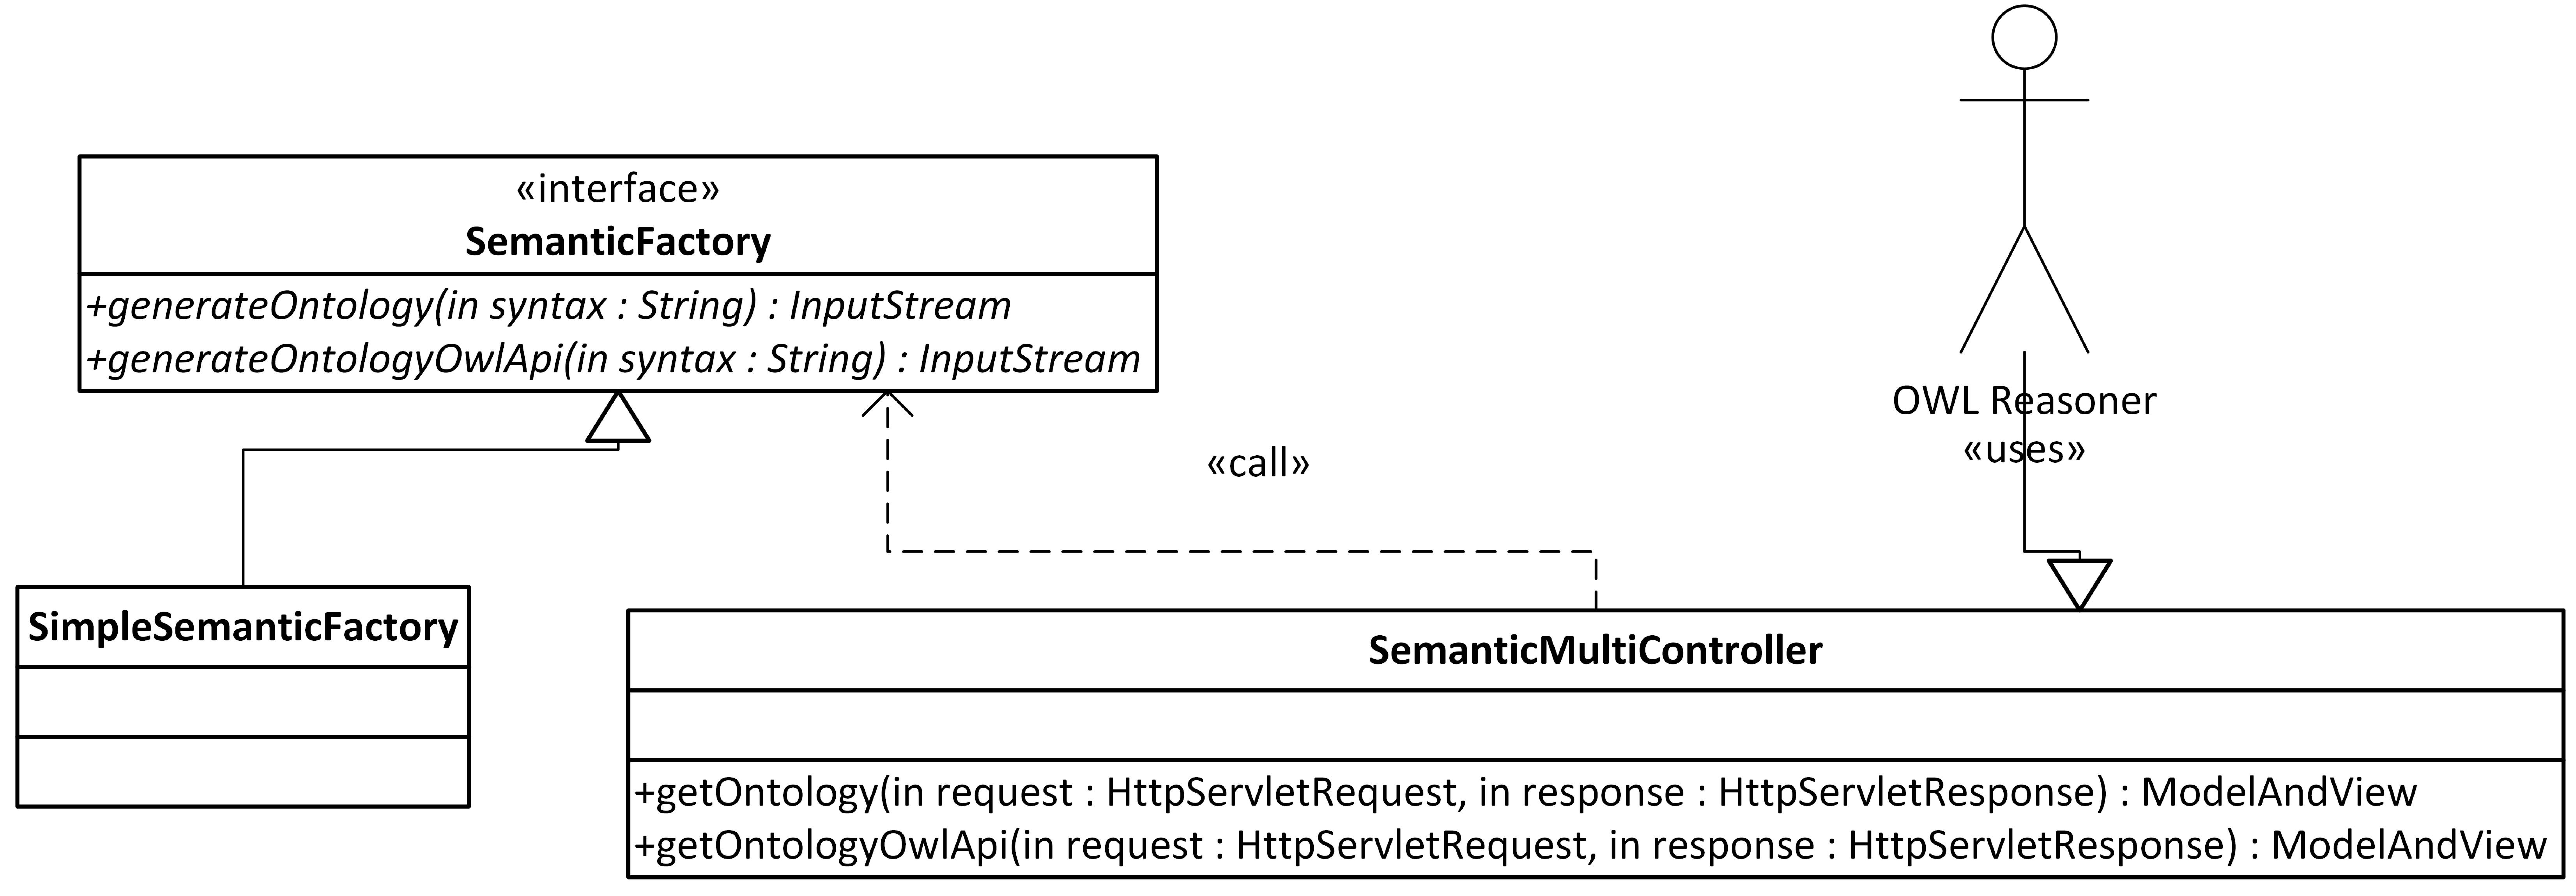
\includegraphics[width=17cm]{SF_integration}
\caption{Semantic Framework Integration. A user (OWL reasoner) calls the \emph{SemanticMulticontroller}. This controller has two methods, \emph{getOntology} and \emph{getOntologyOwlApi}. These methods have one input parameter \emph{type} representing a required output syntax. The Semantic Framework is called through \emph{SemanticFactory} Interface.}
\label{fig:Semantic_Framework_Integration}
\end{figure}

The temporary file is further serialized into a desired syntax. Syntaxes \emph{RDF/XML}, \emph{OWL/XML}, \emph{RDF/XML-ABBREV}, \emph{N-TRIPLE}, \emph{TURTLE}, \emph{N3}, \emph{N3-PP}, \emph{N3-PLAIN}, and \emph{N3-TRIPLE} are currently supported. The \emph{SemanticMultiController} is listening on a specific URL with a \emph{GET} parameter. For instance, when a reasoner visits the URL \emph{http://eegdatabase.kiv.zcu.cz/seman tic/getOntology.html?type=turtle}, it obtains the OWL document in the \emph{turtle} syntax. The UML diagram describing the Semantic module API in the EEG/ERP Portal is shown in Figure \ref{fig:Semantic_Framework_Integration}.

\subsection{Registration within the Neuroscience Information Framework}
\label{Registration_within_nif}

The approach described enables us to generate an experimental ontology from stored experiments. The output ontology is valid according to W3C specification that proves its visualization in Prot\'{e}ge (shown in Figure \ref{fig:visualized_portal_ontology}). To give the ontology a practical sense, we were looking for a suitable authority capable of searching within the ontology.

We successfully used the Neuroscience Informational Framework (NIF) \citep{NIF-Neuroinformatics}. The NIF provides a unified interface for accessing neurophysiological data through resources described by ontology web languages \citep{springerlink:10.1007/s12021-008-9033-y}. NIF uses the proprietary framework \emph{DISCO} \citep{Marenco2010}. It is an XML-based script containing a static description of the registered resource. The dynamic content is accessed through a generated ontology. The structure of metadata instances is stored in an \emph{Interoperability XML} file that is a part of the DISCO protocol. The Interoperability file is stored in the root directory of the EEG/ERP Portal together with generated DISCO files. The NIF reloads it at regular intervals. It enables dynamic access to the dynamic content of the EEG/ERP Portal. Figure \ref{fig:NIF_registry_preview} shows experiments listed through the NIF registry. Currently more then 100 experiments are available and new ones are gradually being added.

\begin{figure}
\center
  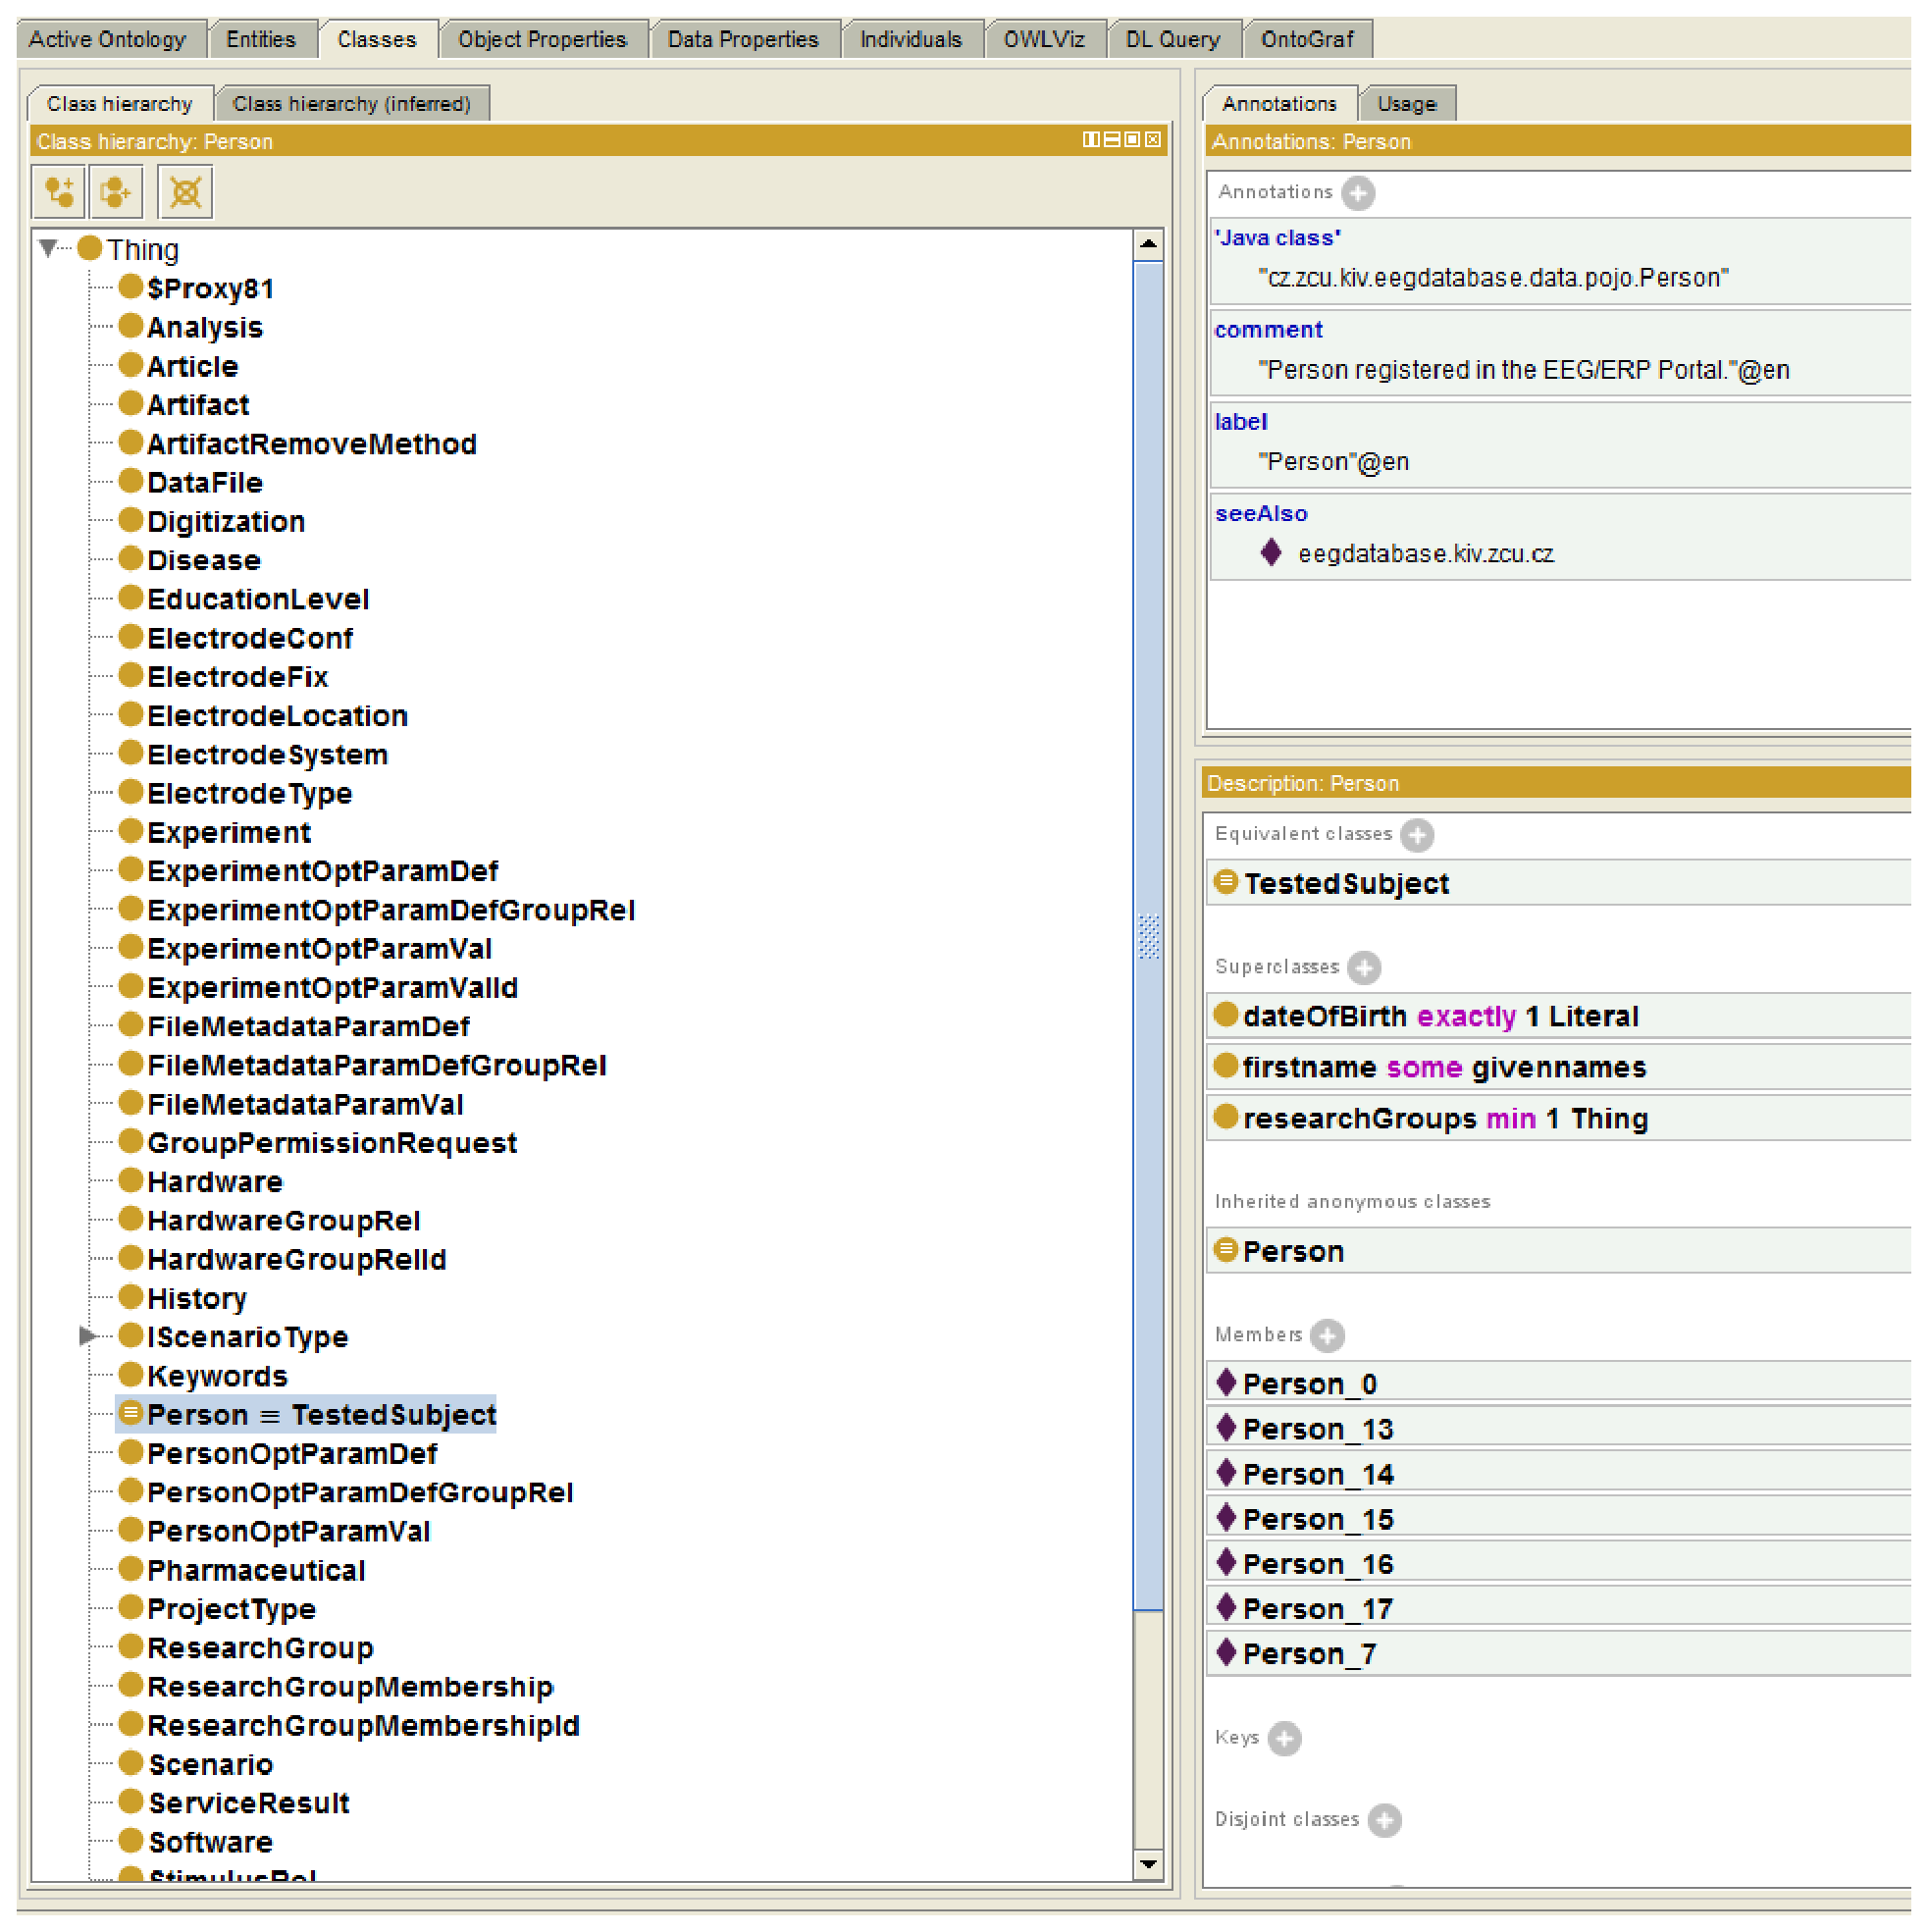
\includegraphics[width=17.5cm]{protege_loaded_ontology}
\caption{Prot\'{e}ge Visualization. The left column shows ontology classes. All classes are subclasses of a superclass \emph{Thing}. The right upper window shows the marked class \emph{Person} and its instances are in the bottom window. The middle window on the right side shows descriptions of annotations transformed from enriched JavaBean. \emph{A Comment} with the value  \emph{"Persons registered in the EEG/ERP Portal"}, and a \emph{label} with the value \emph{"Person"} together with its language mutation are defined in this illustrative example. The class contains an \emph{EquivalentClass} with the value \emph{"TestedSubject"} and a set of restrictions. They define that \emph{DateOfBirth} is present exactly once, the attribute \emph{firstname} is a literal from a list of \emph{given names} and each person is a member of at least one research group.}
\label{fig:visualized_portal_ontology}
\end{figure}

\begin{landscape}
\begin{figure}
  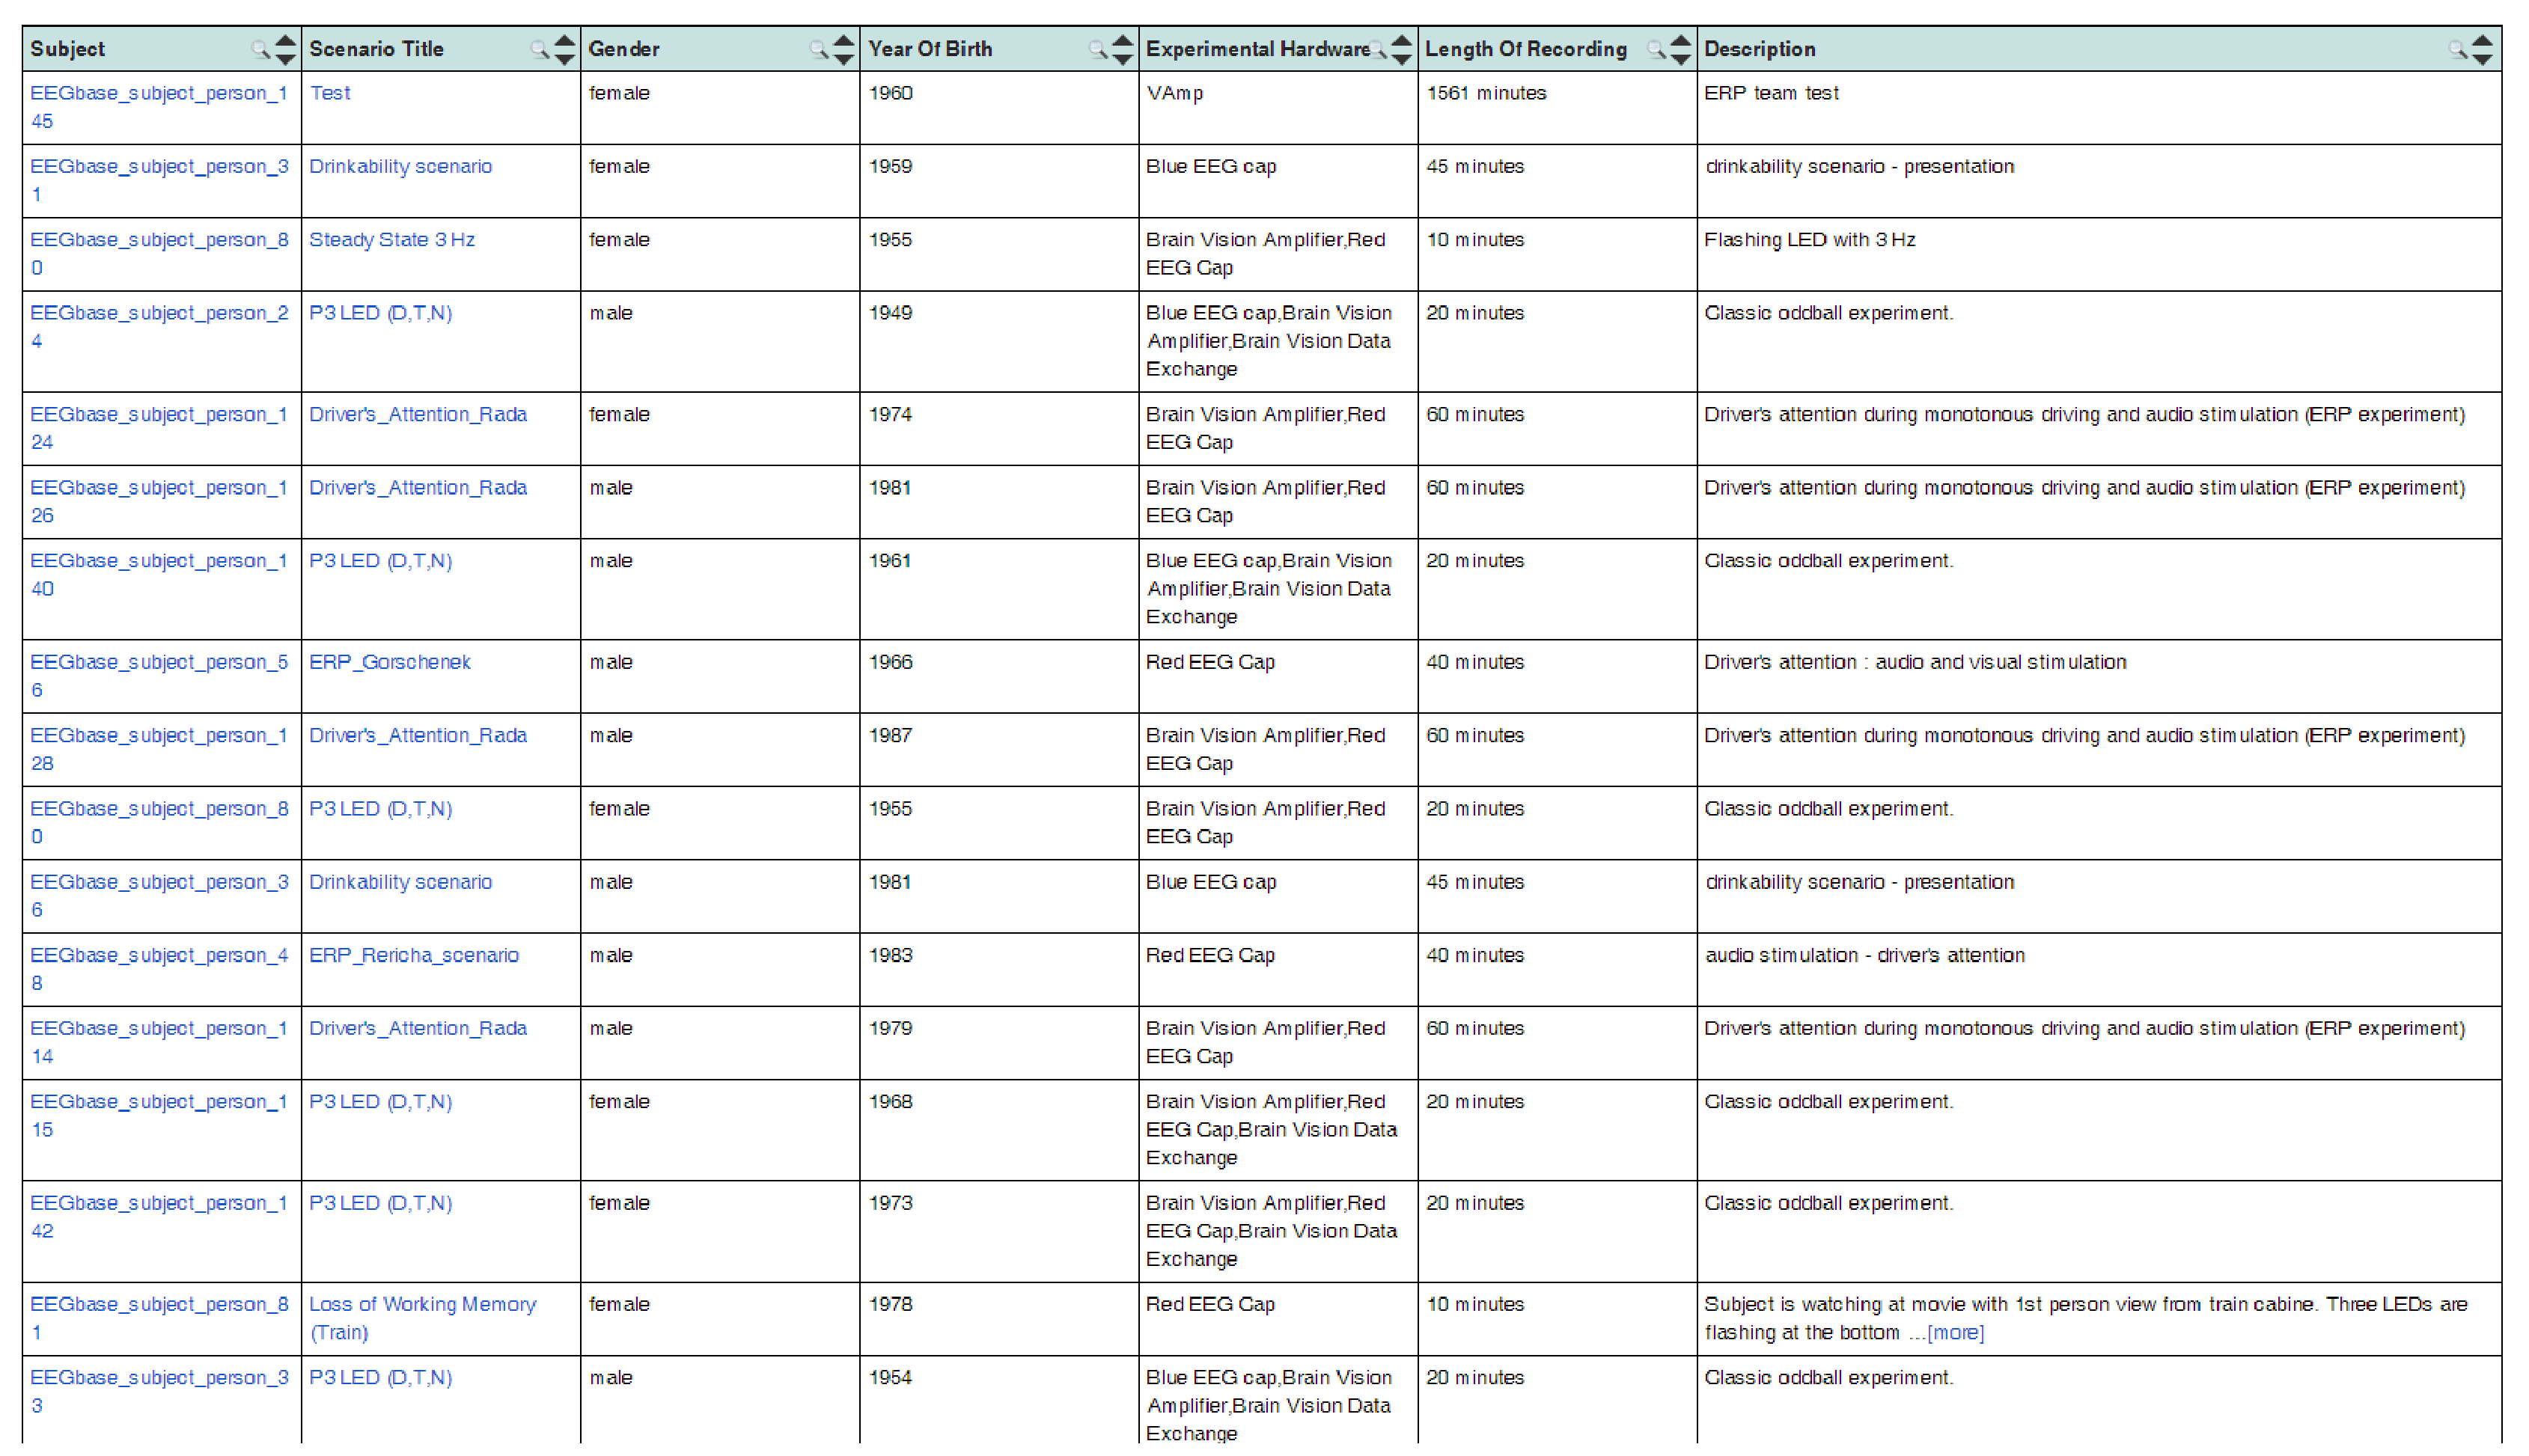
\includegraphics[width=22cm]{nif_preview}
\caption{EEG/ERP Portal in the NIF Registry. The list of experiments stored in the EEG/ERP Portal is shown in the NIF registry at link \protect\url{https://www.neuinfo.org/mynif/search.php?q=eegbase&t=indexable&list=cover&nif=nif-0000-08190-1}. The list contains direct hyperlinks to the experiments stored in the EEG/ERP Portal. When a user click's on a hyperlink, he/she is redirected to the EEG/ERP Portal.}
\label{fig:NIF_registry_preview}
\end{figure}
\end{landscape}


\section{Future Work}
\label{Future_Work}

Since many limitations of OWL exist, its extension OWL2 has been developed. OWL2 aims are to remove different syntaxes, improve datatype expressivity, provide better organization of imports and remove difficulties with different versions of OWL syntaxes. The next significant step we plan is to start with transformation from the object-oriented code into the OWL2 syntax.

Relational-databases are proving inflexible when structure modifications are required because a fixed schema organized in tables is required. NoSQL databases provide higher scalability and availability than relational databases because they are schema-free. When NoSQL databases have key-value organization, they can easily store RDF triples \citep{Papailiou:2012:HAQ:2187980.2188058}. The big challenge lies in the usage of a NoSQL database for storing experimental metadata. There are initiatives (e.g. \citep{Combining-Relational-and-Semi-structured-Databases-for-an-Inquiry-Application}) that investigate the transformation of a common relational database to a NoSQL database. The use of a NoSQL database for electrophysiology experiments should be considered.

The working group at our department is cooperating on the development of a standardized electrophysiology ontology \citep{OEN}. When this ontology is finished, the metadata layer of the EEG/ERP portal will be modified to correspond to this ontology.


\section{Conclusion}
\label{Conclusion}

The approach presented combines ontology development research with classical software programming. While description of a specific electrophysiological domain with specific ontologies is a promising way to share experimental data among laboratories, the software systems are usually implemented using object-oriented programming languages. In addition, these systems are typically developed by software engineers but not semantic web experts. The crucial task is investigating a bridge between object-oriented systems and ontology-based systems.

As a starting point we selected a typical object-oriented system that we mapped to Semantic Web languages.

The most important contribution is a transformational mechanism that maps common JavaBeans into OWL individuals. In addition, the semantic diversity that exists due to different semantic expressivity of the object-oriented code and the Semantic Web languages was partly addressed using a custom annotation-based approach. The proposed transformational mechanism was practically implemented in the Semantic Framework. This framework is a single library usable in domain-independent Java-based systems.

The practical contribution of the approach presented is validated by the registration of the developed EEG/ERP Portal within the Neuroscience Information Framework. The integration of the Semantic Framework enables dynamic generation of the output ontology document. When the ontology document is searchable through the NIF, validity of the approach presented is evaluated.
The ontology registered in NIF enables simple sharing of stored experiments.

Although the presented approach was demonstrated and validated on the electrophysiology domain the mapping mechanism implemented in the Semantic framework is not bound with this domain. It can be used in domain-independent systems.

\section{\uppercase{Acknowledgements}}\label{acknowledgements}

This work was supported by the European Regional Development Fund (ERDF), Project "NTIS - New Technologies for Information Society", European Centre of Excellence, CZ.1.05/1.1.00/02.0090.

%\section{Information Sharing Statement}
%\label{Information_sharing_statement}

%The tools, including the EEG/ERP Portal and the Semantic Framework, are distributed under the GNU Public License. Both are hosted in GitHub repositories. The EEG/ERP Portal is under the INCF group (\url{https://github.com/INCF/eeg-database}) and the Semantic Framework is under the neuroinformatics group of our department (\url{https://github.com/NEUROINFORMATICS-GROUP-FAV-KIV-ZCU/Semantic-Framework}). The EEG/ERP Portal is available on \url{http://eegdatabase.kiv.zcu.cz}.

\bibliographystyle{frontiersinSCNS&ENG} % for Science and Engineering articles
%\bibliographystyle{frontiersinMED} % for Medicine articles
\bibliography{semantic-framework}

\end{document}
